%% LaTeX2e class for student theses
%% sections/content.tex
%% 
%% Karlsruhe Institute of Technology
%% Institute for Program Structures and Data Organization
%% Chair for Software Design and Quality (SDQ)
%%
%% Dr.-Ing. Erik Burger
%% burger@kit.edu
%%
%% Version 1.2, 2016-09-20


\chapter{Integration Process}
\label{ch:ew}

\section{Overview}
A total of 6 multi-chip modules (MCM) were manufactured for the realization of the experimental work of this thesis. The manufacturing and processing of the MCM is detailed thoroughly, especially at the points where modifications were done in order to improve device performance. An overview of each step is outlined throughout this section, with details on the implementation and the setups used in each process. 

\section{Process Flow}

\begin{figure}[!ht]
  \centering
  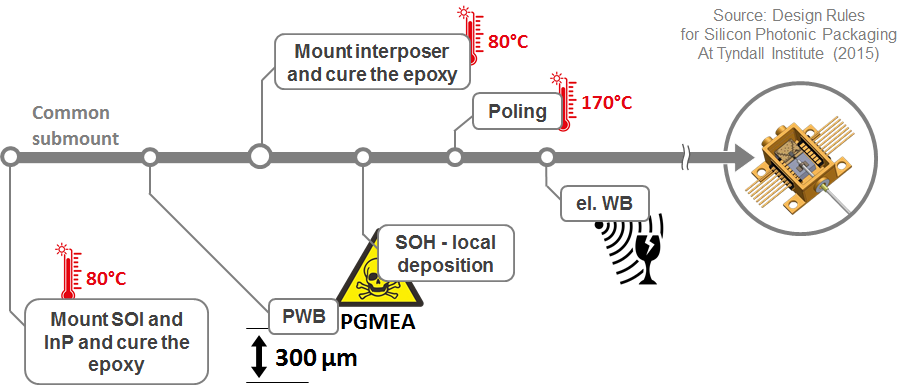
\includegraphics[width=0.9\textwidth]{visio/ProcessFlow_Rastko}
  \caption{Integration process flow for an optically-integrated multi-chip module. The laser and SOH are mounted and fixed to a common submount. The PWB is written in the SOH and the polymer is developed. The EO polymer is locally deposited in the SOH and the polymer is developed. Finally, the EO polymer is poled and the device is optically packaged.  Adapted from \cite{SOHPajkovic16}.}
  \label{fig:PF_R}
\end{figure}

The initial process flow was proposed by Pajkovi{ć} \cite{SOHPajkovic16} and is shown in figure \ref{fig:PF_R}. The scope of that thesis, though, included electrical integration as well, which is not included in the present work in order to constraint the focus to the optical integration process. The process is detailed step-by-step in figure\ref{fig:PF_O}. A color coude showing 

\begin{figure}[!ht]
  \centering
  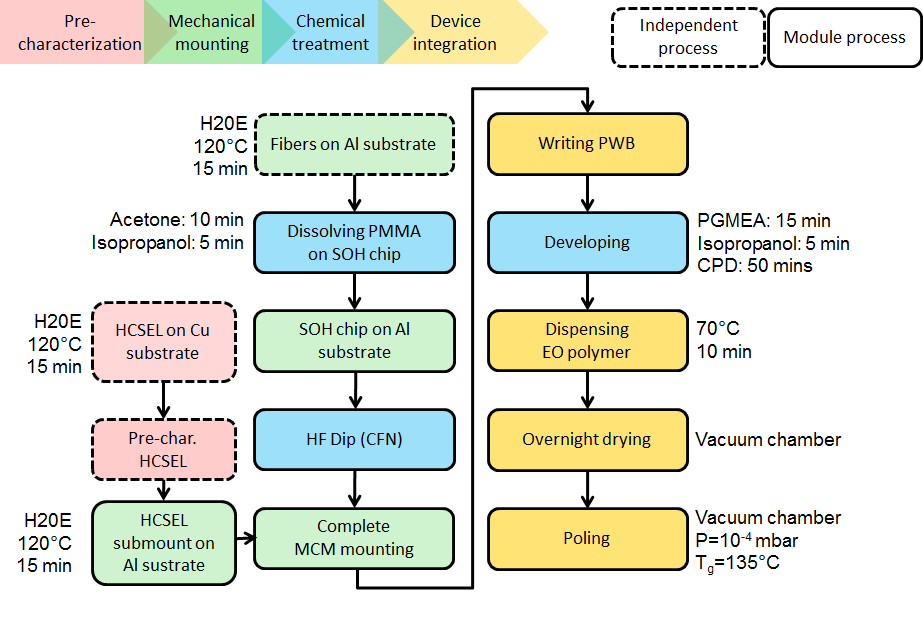
\includegraphics[width=0.95\textwidth]{visio/ProcessFlow_Otorres}
  \caption{Initial integration process flow for an optically-integrated multi-chip module.}
  \label{fig:PF_O}
\end{figure}

\begin{itemize}
\item The HCSEL and SOH chips are pre-characterized to check for HCSEL operation conditions and passive transmission through the SOH. Due to the small footprint of the HCSEL, a spacer slab must be used to facilitate the HCSEL handling as well as a thermal heat sink. Epoxy is used to fix the HCSEL to the spacer and cured by direct heat application using a hot plate.
\item An aluminum submount is used as the common carrier that holds the output single mode fibers, the SOH and the HCSEL.
	\begin{itemize}
	\item The fibers are mounted and attached to the aluminum substrate using epoxy and cured by direct heat application using a hot plate.
	\item The SOH has a protective PMMA layer which is dissolved with acetone by dipping the chip for 10 minutes and washed out with isopropanol. 
	\item The SOH is mounted in the aluminum substrate and fixed with heat-cured epoxy.
	\item The whole module is dipped in hydrofluoric acid (\ce{HF}) to remove the protective \ce{SiO2} layer inside the slot.
	\end{itemize}
\item IP-dip is deposited in the region where the PWBs have to be written and processed by the 3D-micro-lithography printer developed by Nanoscribe. 
\item The PWBs are developed in the clean room using the following steps:
	\begin{itemize}
		\item The module is dipped in PGMEA for 15 minutes, to remove the IP-dip that is not polymerized. 
		\item The module is dipped in isopropanol for 5 minutes to remove any remainders of PGMEA or IP-dip and processed in the critial point dryer (CPD) to avoid strain in the developed PWB due to critical phase change of the isopropanol during drying for 50 minutes.
	\end{itemize}
\item The module is transferred for local deposition of the EO polymer in the slot. After deposition, the device is immediately dried for 10 minutes at \SI{80}{\celsius}.
\item The EO polymer is dried overnight (or for a relatively larger time) in vacuum as a safety buffer to prevent any possible external agents inside the slot.
\item The EO polymer is poled at a pressure of approximately \SI{1e-4}{\milli\bar} and at the glass transition temperature of the EO polymer of \SI{135}{\celsius}.
\end{itemize}

The glue used for fixing all the chips is EPO-TEK\circledR H20S electrically conductive silver epoxy for die stamping. The curing is done by thermal exposure of the common carrier substrate by applying heat using a hot plate at \SI{125}{\celsius} for 15 to 20 minutes. After these steps are completed, the multi-chip module is ready for characterization.

\subsection{HCSEL Pre-characterization}

\subsubsection{LI Curve}

For the LI curve pre-characterization of the HCSEL, the simplified setup shown in figure \ref{lcvR2} is used. Two DC probes are used to make the electrical contact of the HCSEL anode and cathode. The DC probes are connected to a DC precision power source, which is connected via GPIB to a computer that controls voltage or current sweeps, depending on the desired application through a single channel; additionally, the current and voltage of an additional channel can be monitored in software. An integrating sphere placed as close as possible to the HCSEL emission window is connected through a dedicated USB link to the PC for measurement of the light output power.  

%\begin{figure}[!ht]
%\centering
%  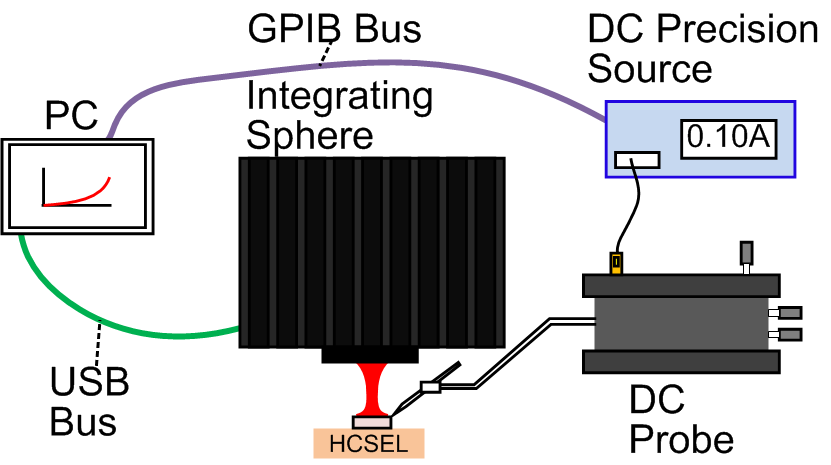
\includegraphics[width=0.8\textwidth]{visio/LIcurve}
%  \caption{LI curve measurement setup.}
%  \label{fig:LIcurve-SU}
%\end{figure}

Figure \ref{fig:precharLI} shows a typical, well-behaved HCSEL chip measurement. In general, all HCSELs are expected to have a linear slope efficiency with a slight decrease close to the operation point $i_{op}=\SI{100}{\milli\ampere}$. In few cases, roll-off is observed in single HCSEL units. This phenomenon is further analyzed in the following section. The threshold current $i_\text{th}$ and the operation power $P_\text{op}$ were measured, with fitting curves used to calculate the threshold current. The method to obtain it is based on a linear, first-degree polynomial fitting in the default MATLAB statistics library, which provides 2-digit precision of the threshold current interpolation. Other methods referenced in the literature \cite{HerstensLDchar05} prefer an approximation by using first- or second-order derivative of the LI curve. Due to the stepping precision used during the characterization (\SI{1}{\milli\ampere}/step), the approximation obtained by computational first- and second-order derivative have a limited range and thus not used.

The  LI curve is the most important figure of merit in the pre-characterization phase, since it gives information about the lasing condition of the HCSEL; thermal roll-off (and whether it is sufficient for correct operation of the MCM); and finally maximum output light power at the operation power current (used to calculate the insertion loss of the MZM and the PWB). The spectral analysis is used to further investigate characteristics of the HCSELs and in most cases only a sanity check for the HCSEL status. 

\begin{figure}[!ht]
\centering
\begin{tabular}{cc}
\subfloat[Typical LI curve]{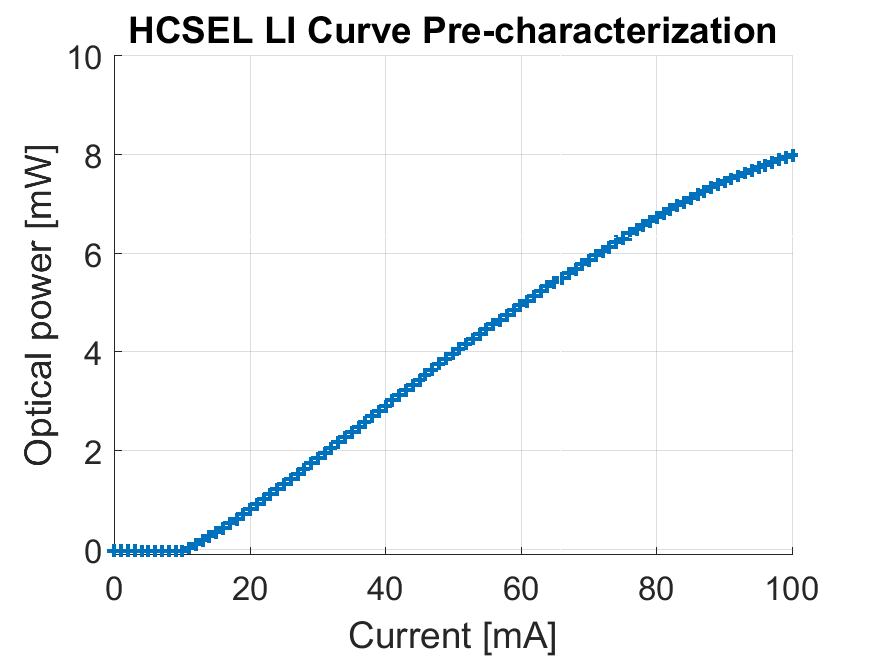
\includegraphics[width=0.45\textwidth,valign=m]{figs/MCM3/LI_laser_ith_iop_demo003}\label{licvR}} &
\subfloat[Measurement setup]{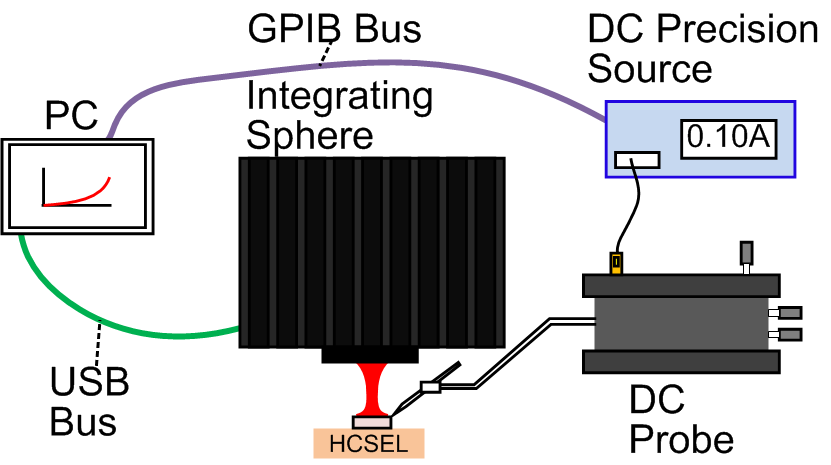
\includegraphics[width=0.45\textwidth,valign=m]{visio/LIcurve}\label{lcvR2}} \\
\end{tabular}
\caption{Measured LI curves. (a) shows the measured LI curve typically measured in a HCSEL device. (b) shows the measurement setup.}
\label{fig:precharLI}
\end{figure}

%\begin{figure}[!ht]
%\centering
%\begin{tabular}{cc}
%\subfloat[Typical LI curve]{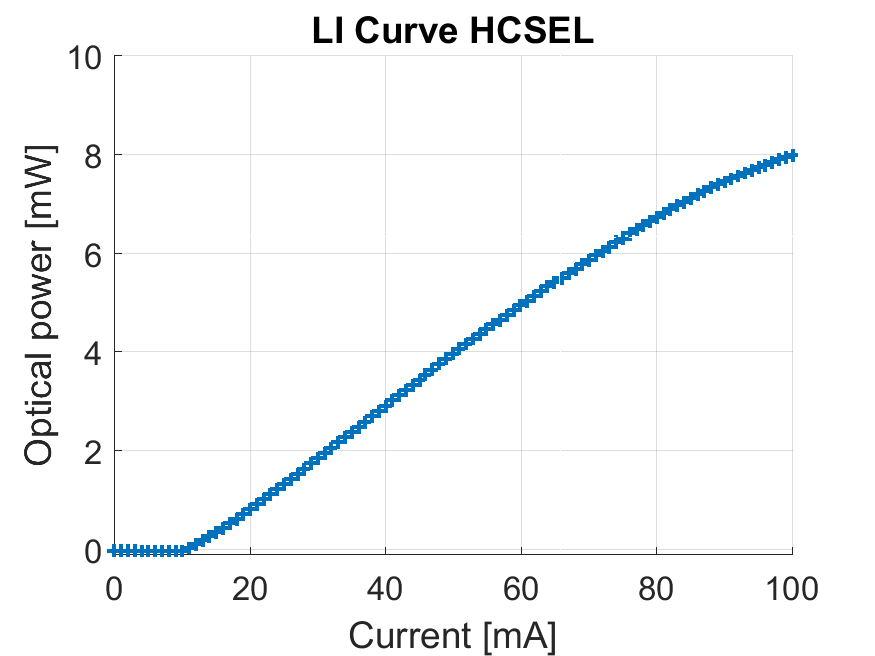
\includegraphics[width=0.45\textwidth]{figs/MCM3/LI_laserA41_2_ith_iop_demo003}\label{licvR}} &
%\subfloat[Threshold fitting]{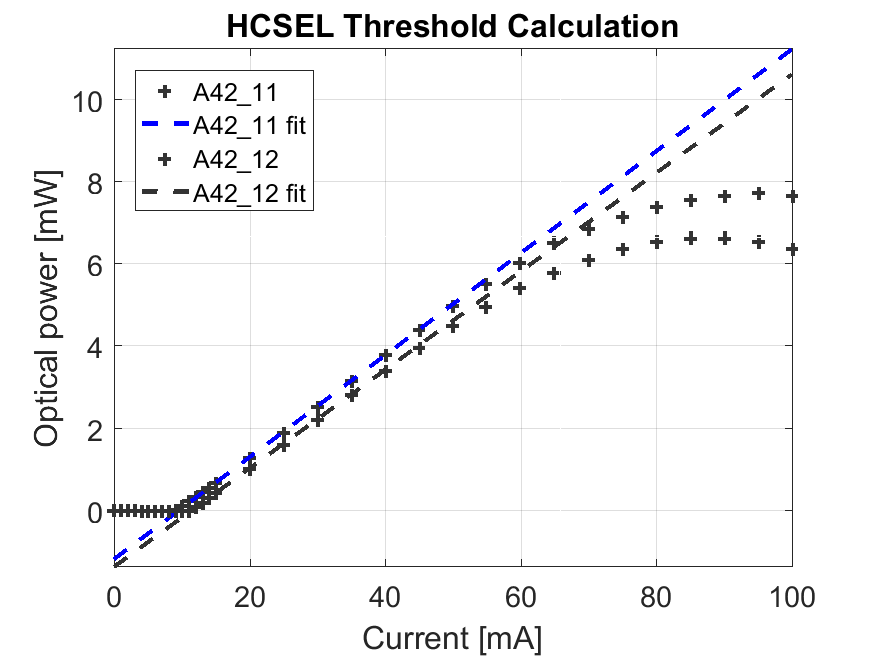
\includegraphics[width=0.45\textwidth]{figs/MCM1/LI_laserA42_ith_demo001}\label{lcvR2}} \\
%\end{tabular}
%\caption{Measured LI curves. Figure \ref{licvR} shows the measured spectrum typically observed in a HCSEL chip. Figure \ref{lcvR2} shows the method used for calculating $i_\text{th}$ of each HCSEL.}
%\label{fig:precharLI}
%\end{figure}



\subsubsection{Spectral curve}

The spectral curves are obtained with the setup shown in figure \ref{fig:SPKcurve-SU}. The DC probes for the LI curve remain unchanged, while the probing part is changed: A coupling fiber which has an adjustable angle $\alpha$ is placed as close as possible to the emission window of the HCSEL, and then divided with a 50:50 beam splitter, with one branch connected to a power meter (to avoid switching between the OSA while doing the fine adjustment of the fiber) and the other connected to the OSA (for the actual measurement of the spectrum). The OSA is calibrated to the wavelength center of the HCSEL at the threshold current and the operation current to have the full wavelength range.

\begin{figure}[!ht]
\centering
\begin{tabular}{cc}
\subfloat[Spectral sweep curve]{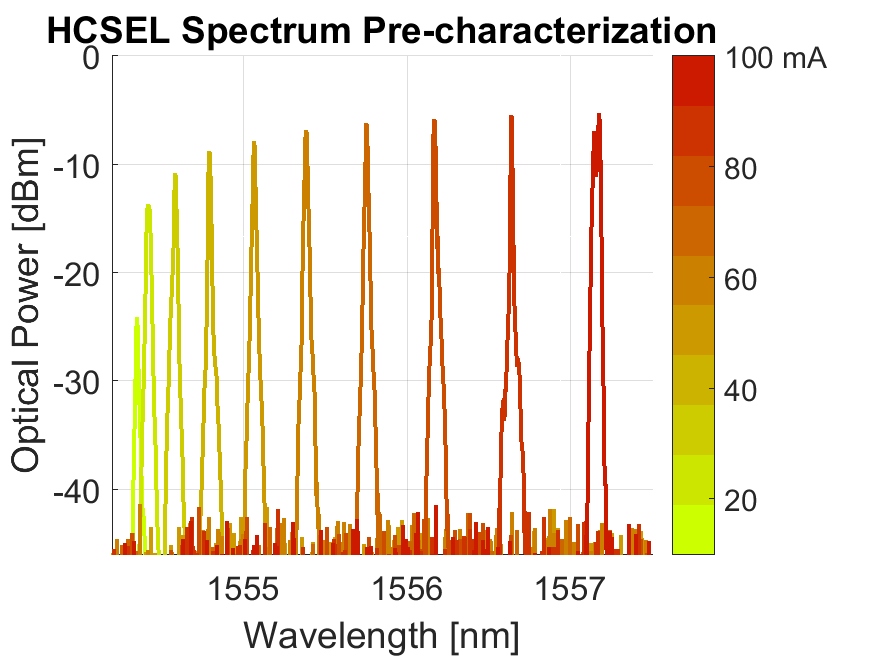
\includegraphics[width=0.45\textwidth,valign=m]{figs/MCM6/SPK/8HCSEL4_Spectrum_demo006_PREx}\label{spkR1}} &
\subfloat[Measurement setup]{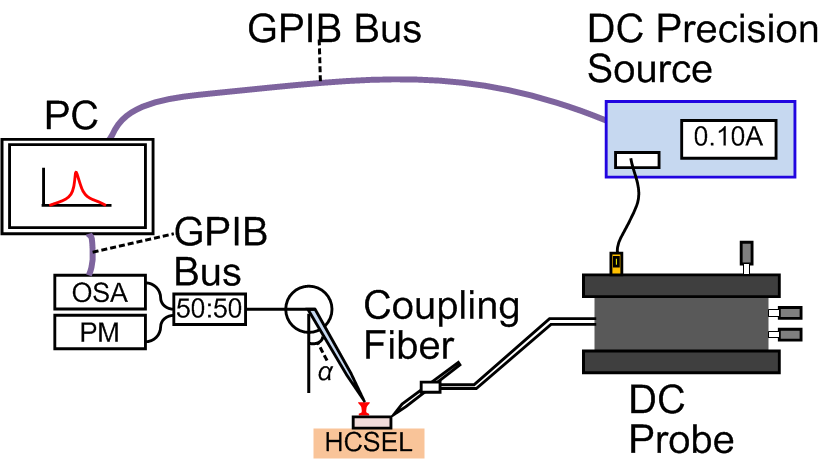
\includegraphics[width=0.45\textwidth,valign=m]{visio/SPKcurve}\label{spkR2}} \\
\end{tabular}
\caption{Measured spectra curves. (a) shows the measured spectra typically measured in a HCSEL device. (b) shows the measurement setup.}
\label{fig:precharSPK}
\end{figure}

%\begin{figure}[!ht]
%\centering
%  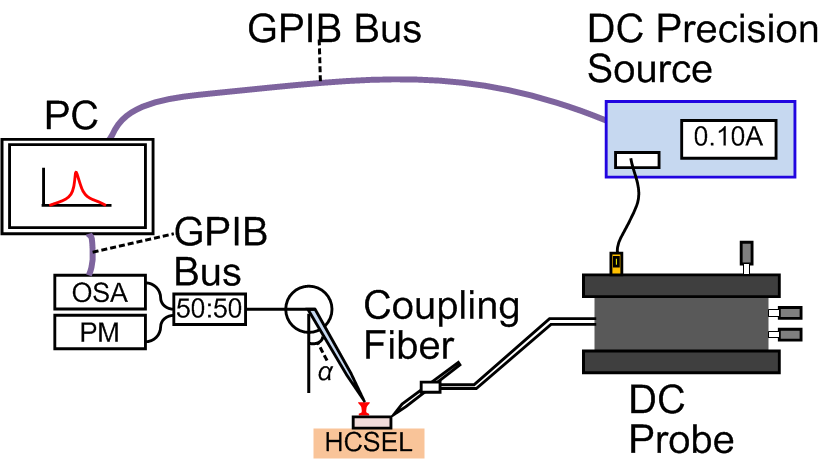
\includegraphics[width=0.7\textwidth]{visio/SPKcurve}
%  \caption{Spectrum curve measurement setup.}
%  \label{fig:SPKcurve-SU}
%\end{figure}

A well-behaved spectrum is shown in figure \ref{spkR2}. The spectrum shifts towards longer wavelengths slightly as current is increased, as predicted before, and it does not show any spectral hole burning and has a monotonic profile. Any possible mode-hopping can be also observed with this measurement, which occurs when the wavelength shift is not monotonically increasing towards redder wavelengths. 

%\begin{figure}[!hb]
%\centering
%  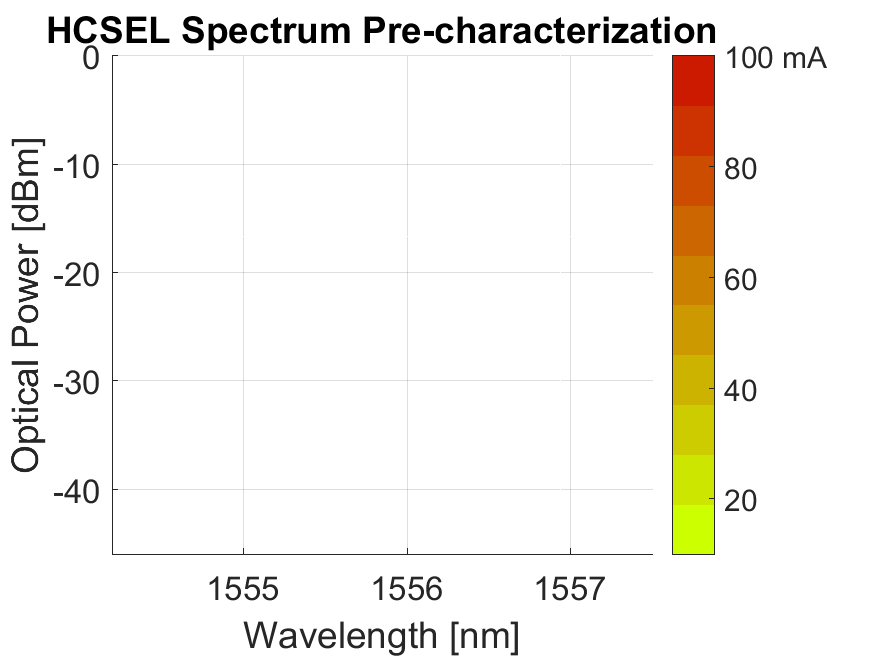
\includegraphics[width=0.8\textwidth]{figs/MCM6/SPK/8HCSEL4_Spectrum_demo006_PRE}
%  \caption{Measured spectrum of HCSEL.}
%  \label{fig:precharSPK}
%\end{figure}

\subsection{Mount Assembly}
\label{sec:exp:massy}

\begin{figure}[!ht]
\centering
  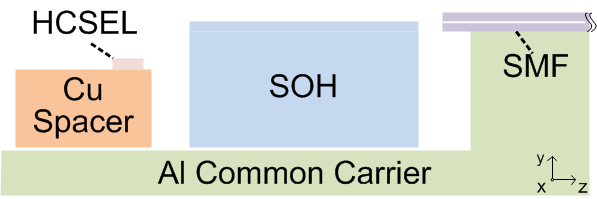
\includegraphics[width=0.65\textwidth]{visio/MCM1-SU}
  \caption{Multi-chip module stack-up. A HCSEL is mounted on a copper spacer submount and glued to a SOH chip on an aluminum common carrier. Single mode fibers are mounted on the common carrier for light outcoupling.}
  \label{fig:MCM1-SUx}
\end{figure}
%\footnote{The laser submount to commonly as ``spacer'' since the laser chip dimensions are much smaller than the SOH substrate and device, hence the additional space to connect the devices through the PWB.}
%\footnote{Width $\times$ Length $\times$ Height}

 \begin{figure}[!ht]
\centering
\begin{tabular}{cc}
\subfloat[Bad spacing]{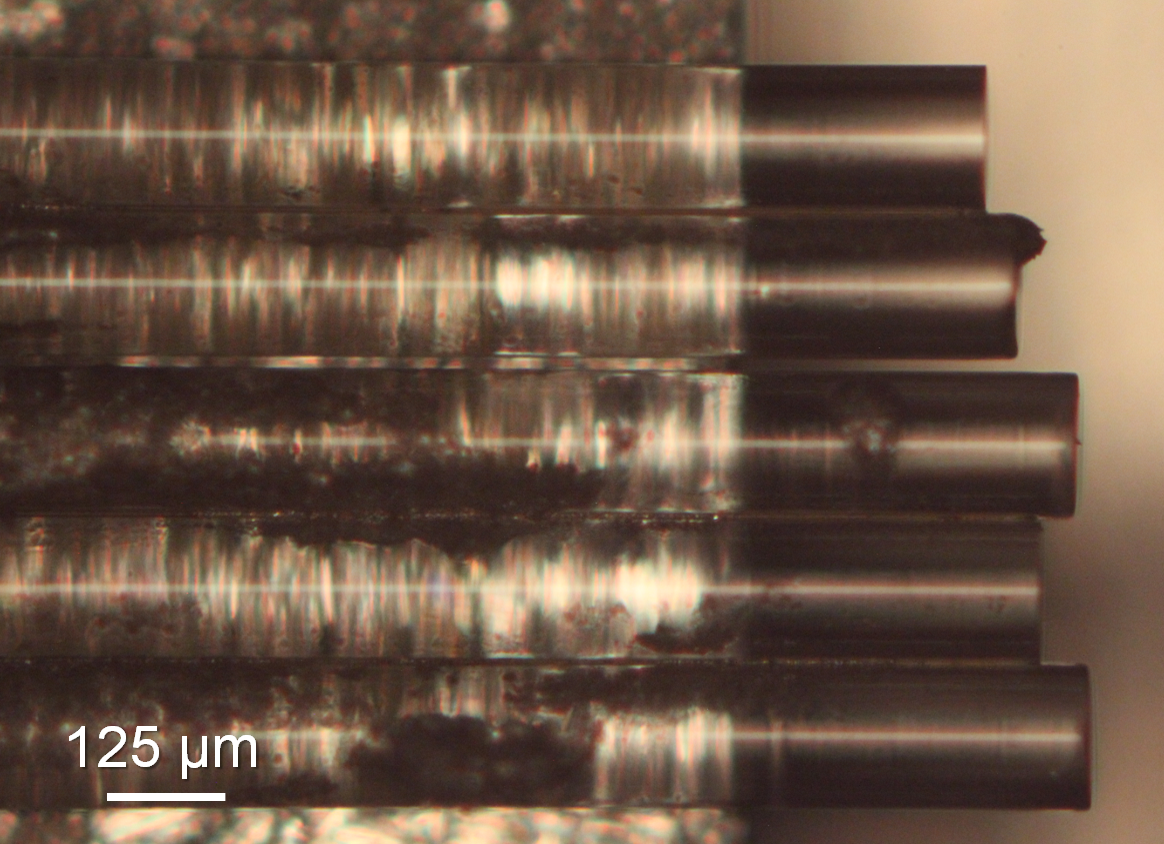
\includegraphics[width=0.46\textwidth,valign=m]{lab/bad_spacing2}\label{fig:badsp}} &
\subfloat[Good spacing]{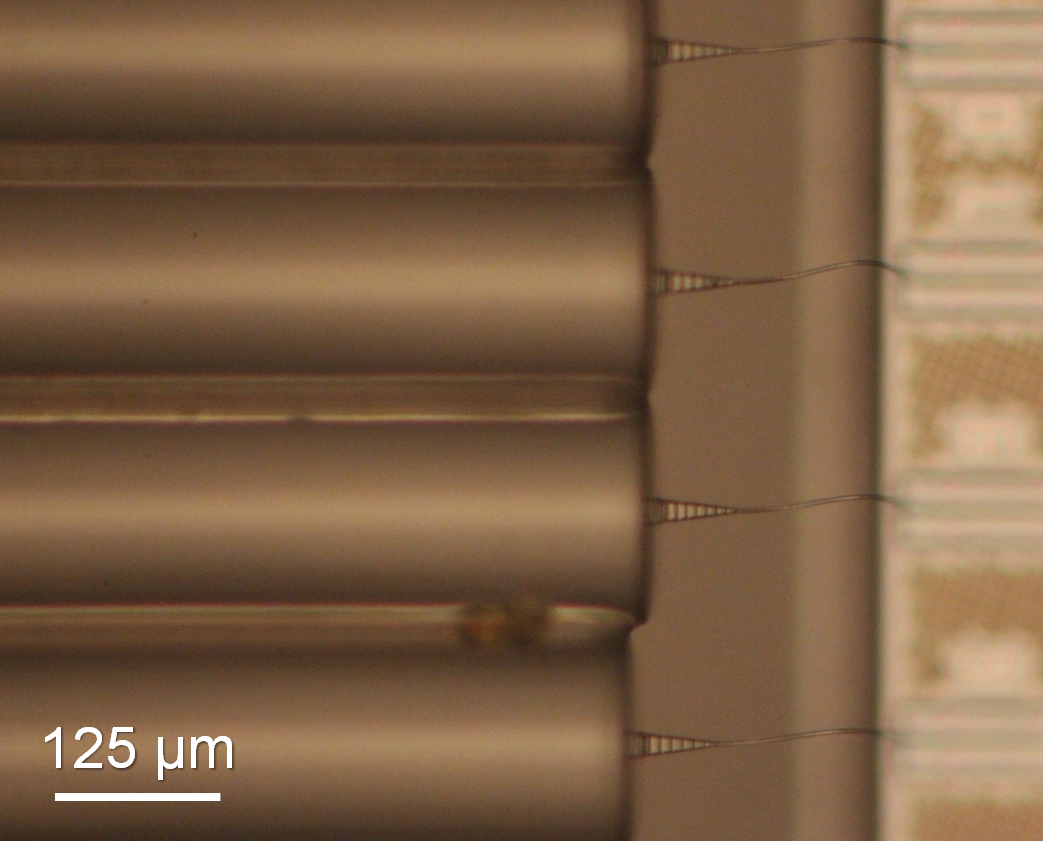
\includegraphics[width=0.41\textwidth,valign=m]{lab/good_spacing}\label{fig:goodsp}} \\
\end{tabular}
\caption{Fiber spacing for PWB writing. (a) shows uneven spacing between fibers. (b) shows even spacing.}
\label{fig:spacing}
\end{figure}


The main mounting substrate is an aluminum common carrier fabricated in-house to design specification as shown in \ref{fig:MCM1-SUx}. The submount (or spacer) used for the laser chip is a copper slab of $\SI{4}{\milli\meter} \times \SI{2}{\milli\meter} \times \SI{0.5}{\milli\meter}$. The SOH modulator modules used were the MS3-IME2 BigPipes SOH chip, consisting of 8 \SI{1.5}{\milli\meter} MZMs, 8 input ports, and 8 output single ports and 2 combined output ports; and the MS1-IME2 SOH chip, consisting of 8 \SI{1}{\milli\meter} IQ modulators, with 4 input ports, and 4 combined output ports. The fibers used to connect the SOH modulator are single-mode fibers (SMF) with a cladding size of \SI{125}{\micro\meter}. Naked fiber stubs are used for spacing fibers in the common carrier mount, because the spacing between ports is exactly \SI{125}{\micro\meter}. Special care is taken to avoid overfilling of glue between the fibers, as seen in \ref{fig:badsp}, excess of glue caused a misalignment of the fibers. Even though the misalignment is a few micrometers, it can be seen from the example of good spacing in figure \ref{fig:goodsp}, the optical path of the PWB is more homogeneous under equal spacing, so the loss analysis can be simplified for multiple devices.
 
%\clearpage %to make it cleaner in the output file

\subsection{PWB Fabrication}
\label{sec:exp:PWB}

\begin{figure}[!ht]
\centering
  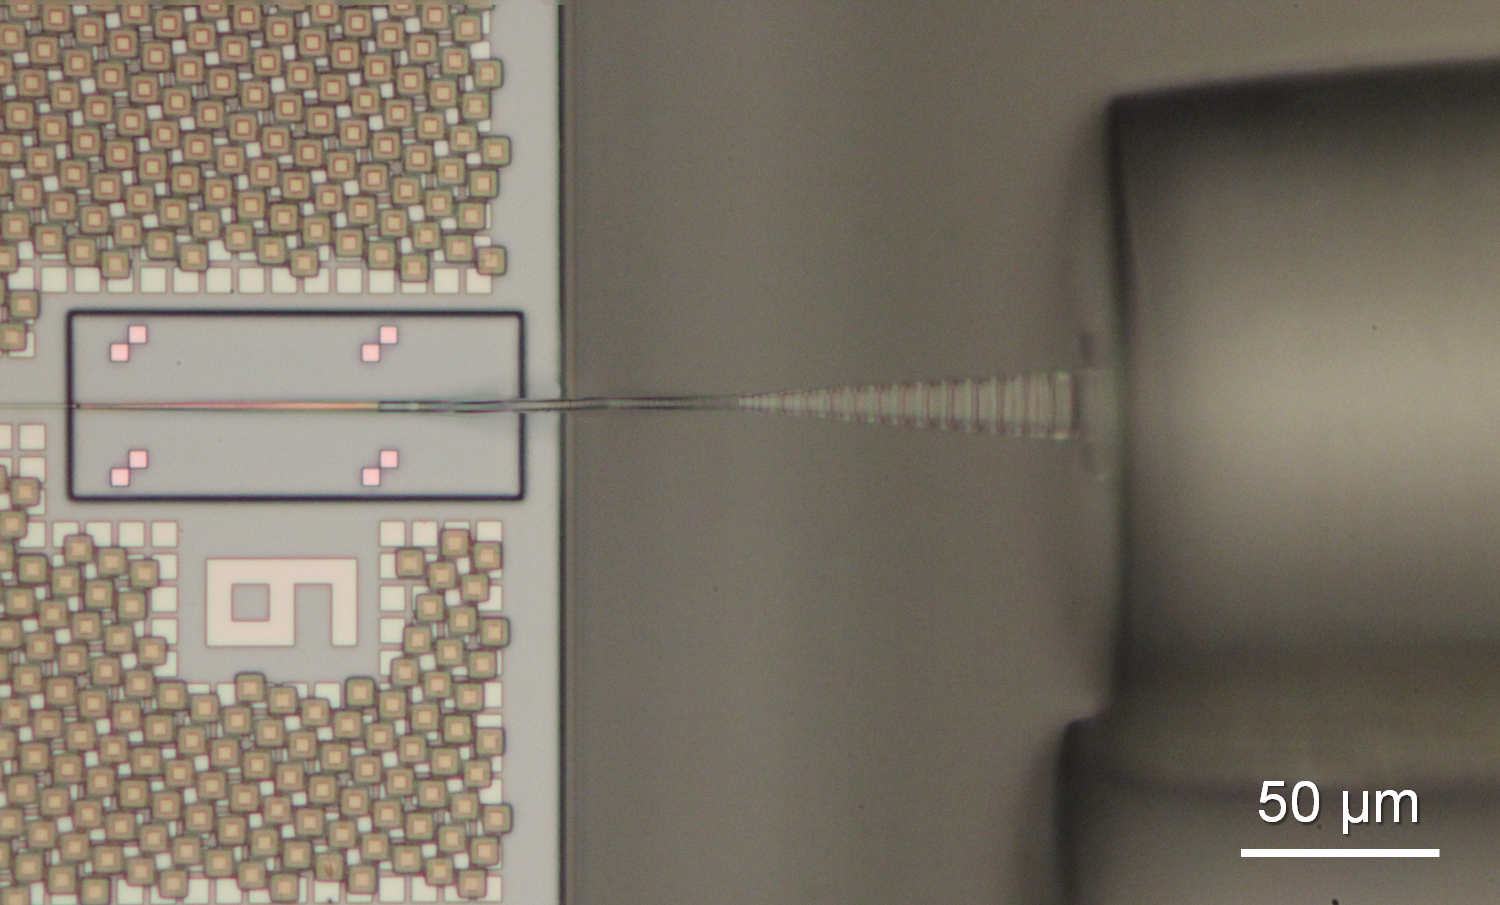
\includegraphics[width=0.7\textwidth]{lab/PWB_comp1_red}
  \caption{Composite image of PWB on the fiber side.}
  \label{fig:PWB_comp}
\end{figure}

The fabrication process of the PWB is followed as already discussed in section \ref{ch:th:fabPWB}, and then analyzed using a microscope to observe specific details of the PWB.  Figure \ref{fig:PWB_comp} shows a composite image of a PWB written on a MCM. The image is composed of several focal depths since there is a slight height difference between the fiber and the SOH chip.

 \begin{figure}[!ht]
\centering
\begin{tabular}{cc}
\subfloat[Emission window]{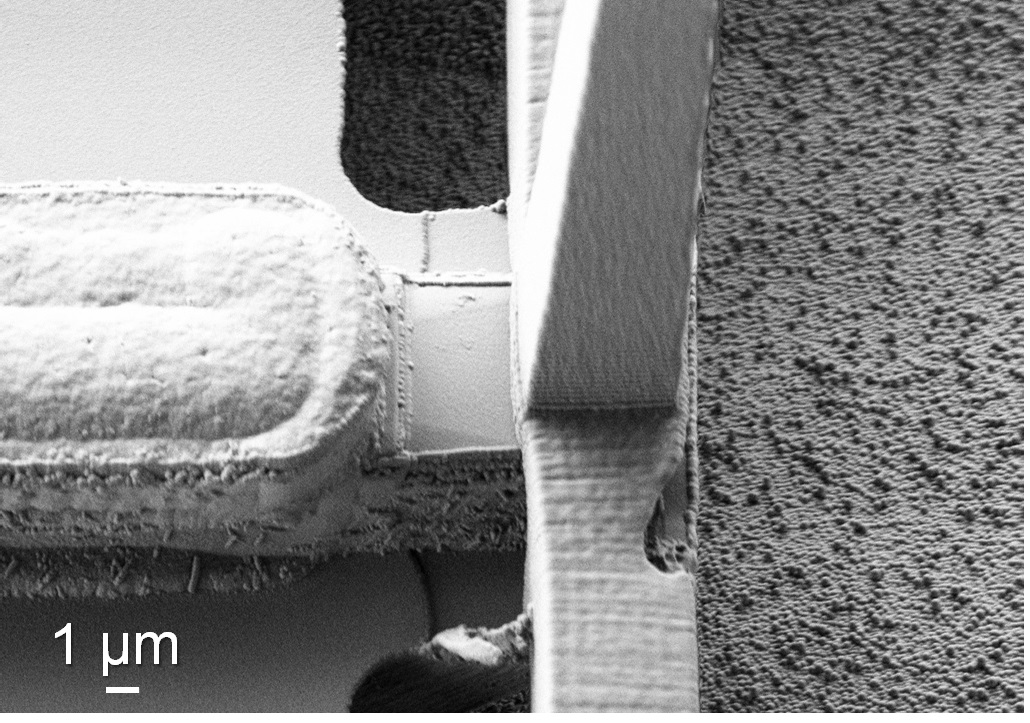
\includegraphics[width=0.45\textwidth,valign=m]{lab/SOH_MCM_SEM1.jpg}\label{fig:SEM1}} &
\subfloat[\SI{45}{\degree} view of PWB]{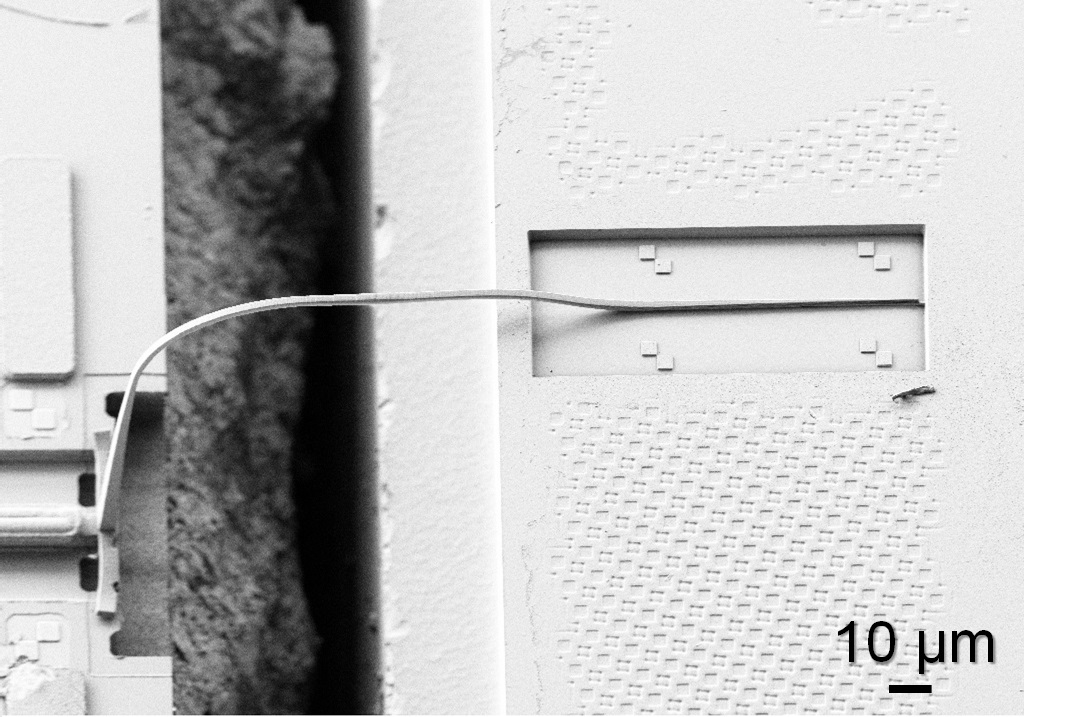
\includegraphics[width=0.45\textwidth,valign=m]{lab/SOH_MCM_SEM2.jpg}\label{fig:SEM2}} \\
\end{tabular}
\caption{SEM pictures of PWB on the HCSEL side.}
\label{fig:SEM}
\end{figure}

The PWBs are also analyzed in their fine structure through scanning electron microscopy (SEM), in order to find artifacts such as micro-explosions (due to laser light over-exposure) or small misalignments close to the taper edges. Figure \ref{fig:SEM} shows an SEM picture of a PWB written on the HCSEL side, showing the detail at the emission window and a rotated view which allows to see the curvature of the PWB into the taper of the SOH. 

\subsection{Local Deposition}
\label{sec:exp:locdepo}

\begin{figure}[!ht]
\centering
  
\includegraphics[width=0.6\textwidth]{visio/LD-SU}
  \caption{Local deposition setup. A ESP300 motion controller is controlled via GPIB through a computer to move in x-, y- and z-axes with \SI{10}{\micro\meter} step precision. Two cameras with objective lenses are used for monitoring in the xy- and z-directions.}
  \label{fig:LD-SU}
\end{figure}

The setup used for local deposition is shown in figure \ref{fig:LD-SU}. The GUI and movement tools was modified during this master thesis and the elements that were updated are documented in \ref{ch:LD}.  After the multi-chip module is placed in the metallic mount, the tilt of the chip is adjusted since small variations in the height of the chip can lead to permanent damage by scratching of the waveguides with the application needle. The EO polymer is applied to the needle after tilt adjustment and locally deposited in all the devices of interest. After the EO polymer is deposited, the device is placed on a hot plate and the polymer is dried for 10 minutes at \SI{80}{\celsius}. The module is placed overnight in a vacuum chamber for the final drying process.

\subsection{Electrical Poling}
\label{sec:exp:epol}
%A simplified schematic setup is shown in figure \ref{fig:poling-SU}.
After local deposition of the organic material, the multi-chip module (MCM) is poled by applying a voltage in the ground terminals (thus exciting an electric field in the waveguide slot). The SOH has four ground terminals wired on-chip on each side of the modulator, thus allowing for parallel poling of four devices at a time; By using two outputs of a variable power source, all 8 devices can be poled at once. The MCM is placed inside a vacuum chamber, in which pressure and temperature can be controlled, with DC probes and plugged through the electrical connector in the chamber that allows for external injection of power to the chip. After the vacuum chamber is closed, the temperature is steadily increased until a temperature of \SI{135}{\celsius} is reached, and an approximate pressure of \SI{1e-4}{\milli\bar} is set. The voltage source is set to reach \SI{48}{\volt}, which for a slit width of \SI{320}{\nano\meter} equates to an electric field of \SI{150}{\volt/\micro\meter}. The temperature is steadily decreased (thus ``freezing'' the state of the organic material dipole moments in the direction of the external electric field) followed by a steady, controlled voltage drop; finally, the vacuum chamber is depressurized and the MCM is cooled down with a peltier device.

%\begin{figure}[!ht]
%\centering
%  \includegraphics[width=0.4\textwidth]{visio/poling-SU}
%  \caption{Poling setup.}
%  \label{fig:poling-SU}
%\end{figure}

\subsection{Optically Packaged Transmitter}

The optically-packaged, fully-processed SOH transmitter is shown in figure \ref{fig:optTX}. A detail of the PWB on both sides of the SOH modulator are also shown, which were taken in order to detect any possible fabrication defects during the PWB processing, some of which can be: Micro-explosions in the development of IP-Dip (due to overexposure of the laser in a specific voxel region); misalignment of the PWB with respect to the reference taper; and PWB curvature (due to miscalculations in the positioning algorithm), to name a few. %The PWB SEM pictures shown have few fabrication defects. 

\begin{figure}[!ht]
\centering
  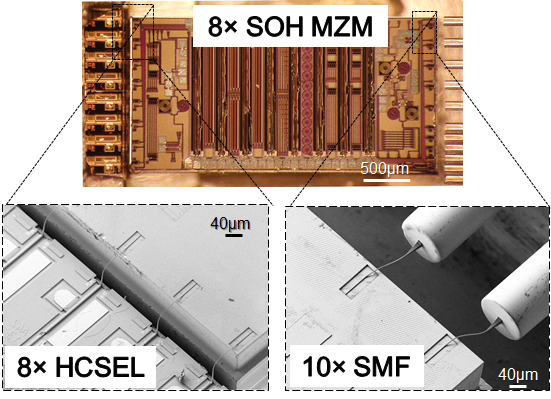
\includegraphics[width=0.7\textwidth]{lab/optTX_v3}
  \caption{Optically packaged transmitter with SEM detail of PWBs on the HCSEL and the SMF side.}
  \label{fig:optTX}
\end{figure}

The following step is the optical characterization of the MCM transmitter, in the following order:

%\footnote{in german literature it is also referred to as $\text{U}_\pi$}
%(typically \SI{313}{\hertz}) 
\begin{itemize}
\item \textbf{$\text{V}_\pi$}: This is commonly measured in a low frequency range and a photodetector or an optical test set in order to convert the optical signal to an electrical signal that can be measured using an oscilloscope. 
\item \textbf{Integrated laser launch power}: It provides the insertion loss of the full optical path in the module (PWB input - MZM - PWB output) using the integrated HCSEL as a light source. The measurement is done directly at the output fibers. A bias voltage is also applied to find the best transmission maximum. A wavelength sweep can be done to find local maxima and minima for unbalanced configurations. In case a strong argument is required to reassure that there is no change in the light power output throughout the processing of the MCM. The performance of the HCSEL can be monitored using the built-in current sensing diode to detect any changes in the operation current. 
\item \textbf{PWB/MZM insertion loss characterization}: Using the grating coupler (GC) inputs and outputs provides the insertion loss of each individual element in the optical path, with the integrated HCSEL and an external tunable laser source (TLS) to form three additional optical paths that allow for interpolating the individual insertion losses of each element through transmission measurements.
%\item \textbf{HCSEL post-processing characterization}: The HCSEL performance can potentially be changed during the process since it undergoes a series of environmental changes, such as temperature, pressure, solution dipping, etc. Thus, a post-processing characterization provides some information if any specific changes that might have occured in the HCSEL.
\end{itemize}

The measurement results for the optical path losses are summarized in table \ref{tab:IL}. A calibration measurement of the back-to-back transmission (TLS-Power meter/OSA) is performed before using the MCM. A measurement of the grating coupler-to-grating coupler (GC-GC) transmission was used as a reference for the calculation of all devices at approximately \SI{10.5}{\decibel} maximum transmission, since fiber couplers measurement setup used throughout the experimental development were not changed (i.e. fiber coupler at \SI{14}{\degree}). The grating coupler transmission was obtained from test structures located on-chip. The transmission of the multimode interferometer power splitters was taken from the results obtained by Rainer \cite{MMIRainer16}, where two optical paths differing by exactly one MMI were measured and a mean value of \SI{3.5}{\decibel} was obtained. The insertion loss of the Mach-Zender modulator is thus approximately 6dB for the C-Band range (\SIrange{1530}{1565}{\nano\meter}). The losses of the PWB were measured as a combined PWB loss for most devices (to reduce possible damage to the PWB and enable data transmission experiment), but single PWB were characterized in a single MCM with the best performing case at \SI{4.9}{\decibel} with air as the overcladding material.

%\begin{figure}[!ht]
%\centering
%  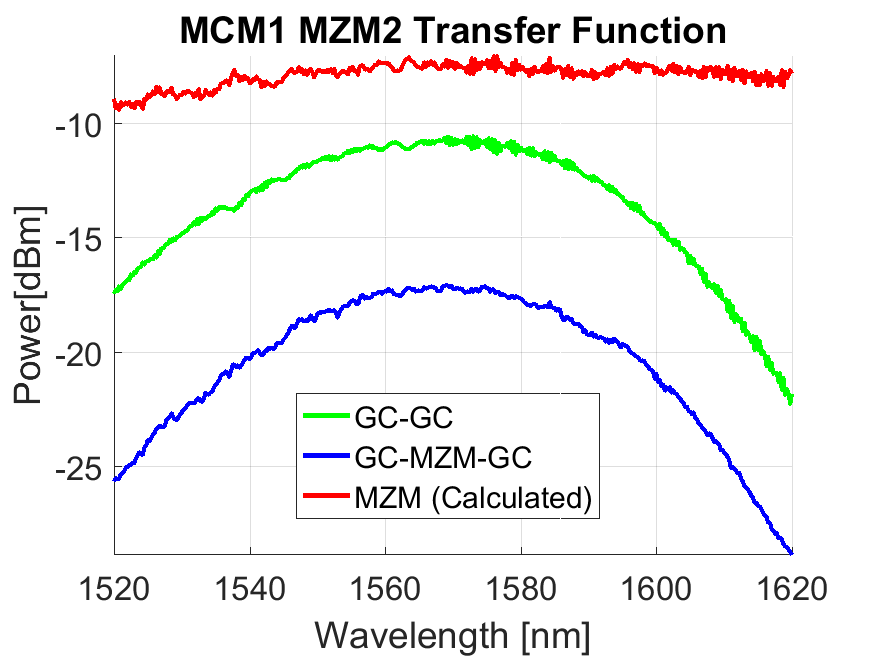
\includegraphics[width=0.7\textwidth]{figs/MCM1/MCM1_MZM2_TC_demo001}
%  \caption{MZM calculated insertion loss.}
%  \label{fig:IL001}
%\end{figure}


%MCM & Device & $P_\text{op}$ & $P_\text{launch}$ & B2B  & GC-GC & GC-MZM-GC & MMI  & MZM & PWB  & PWB1 & PWB2 \\ \midrule
%1   & 2      & 8.04  & -10.5     & -1.0 & -10.5 & -18.5     & 0.0 & 9.0 & 11.5 & 5.7  & 5.7  \\
%4   & 2      & 7.06  & -4.6      & -5.1 & -10.5 & -22.7     & 3.5  & 7.1 & 8.13 & 4.1  & 4.1  \\
%4   & 3      & 6.06  & -4.5      & -5.1 & -10.5 & -21.7     & 3.5  & 6.1 & 8.1  & 4.0  & 4.0  \\
%4   & 4      & 3.96  & -4.4      & -5.1 & -10.5 & -24.2     & 3.5  & 8.6 & 12.5 & 6.2  & 6.2  \\ \bottomrule

% Please add the following required packages to your document preamble:
% \usepackage{booktabs}
\begin{table}[]
\centering
\begin{tabular}{@{}L{2cm}L{1.0cm}L{1.5cm}L{2cm}L{2cm}L{2cm}L{2cm}L{2cm}L{2cm}L{2cm}L{2cm}L{2cm}@{}}
\toprule
Module   & $P_\text{op}$ [dBm] & $P_\text{launch}$ [dBm] & G-M-G [dB]  & Modulator [dB/mm] & $V_\pi \cdot L$ [V$\cdot$mm] & PWB$\times 2$ [dB] \\ \midrule
MZM    & 8.04  & -10.5     &        -18.5    & -6.0 & 1.16 &  -11.4  \\
IQ     & 6.06  & -4.5      &       -21.7      & -6.1 & 1.32 &  -8.0  \\ \bottomrule
\end{tabular}
\caption{Summary of transmission measurements and calculations for best performing MCMs. The table shows the operation power measured in the pre-characterization $P_\text{op}$, the launch power on the fiber side $P_\text{launch}$, the optical path from GC to MZM and GC (G-M-G), the modulator transmission, the $V_\pi$ per unit length and the combined transmission losses of the input and output photonic wire bonds (PWB$\times$2.}
\label{tab:IL}
\end{table}
%$P_\text{op}$ &
%& 8.04
%& 7.06
% & 6.06 
%& 3.96 

%$P_\text{launch}$ &
%& -10.5
% & -4.6 
%  & -4.5 
%& -4.4 

\section{Process Flow Modifications}
\label{sec:Evaluation:mfg}

%\begin{figure}[!ht]
%\centering
%\begin{tabular}{cc}
%\subfloat[Broken tapers]{{\label{fig:mcm1_AS1}}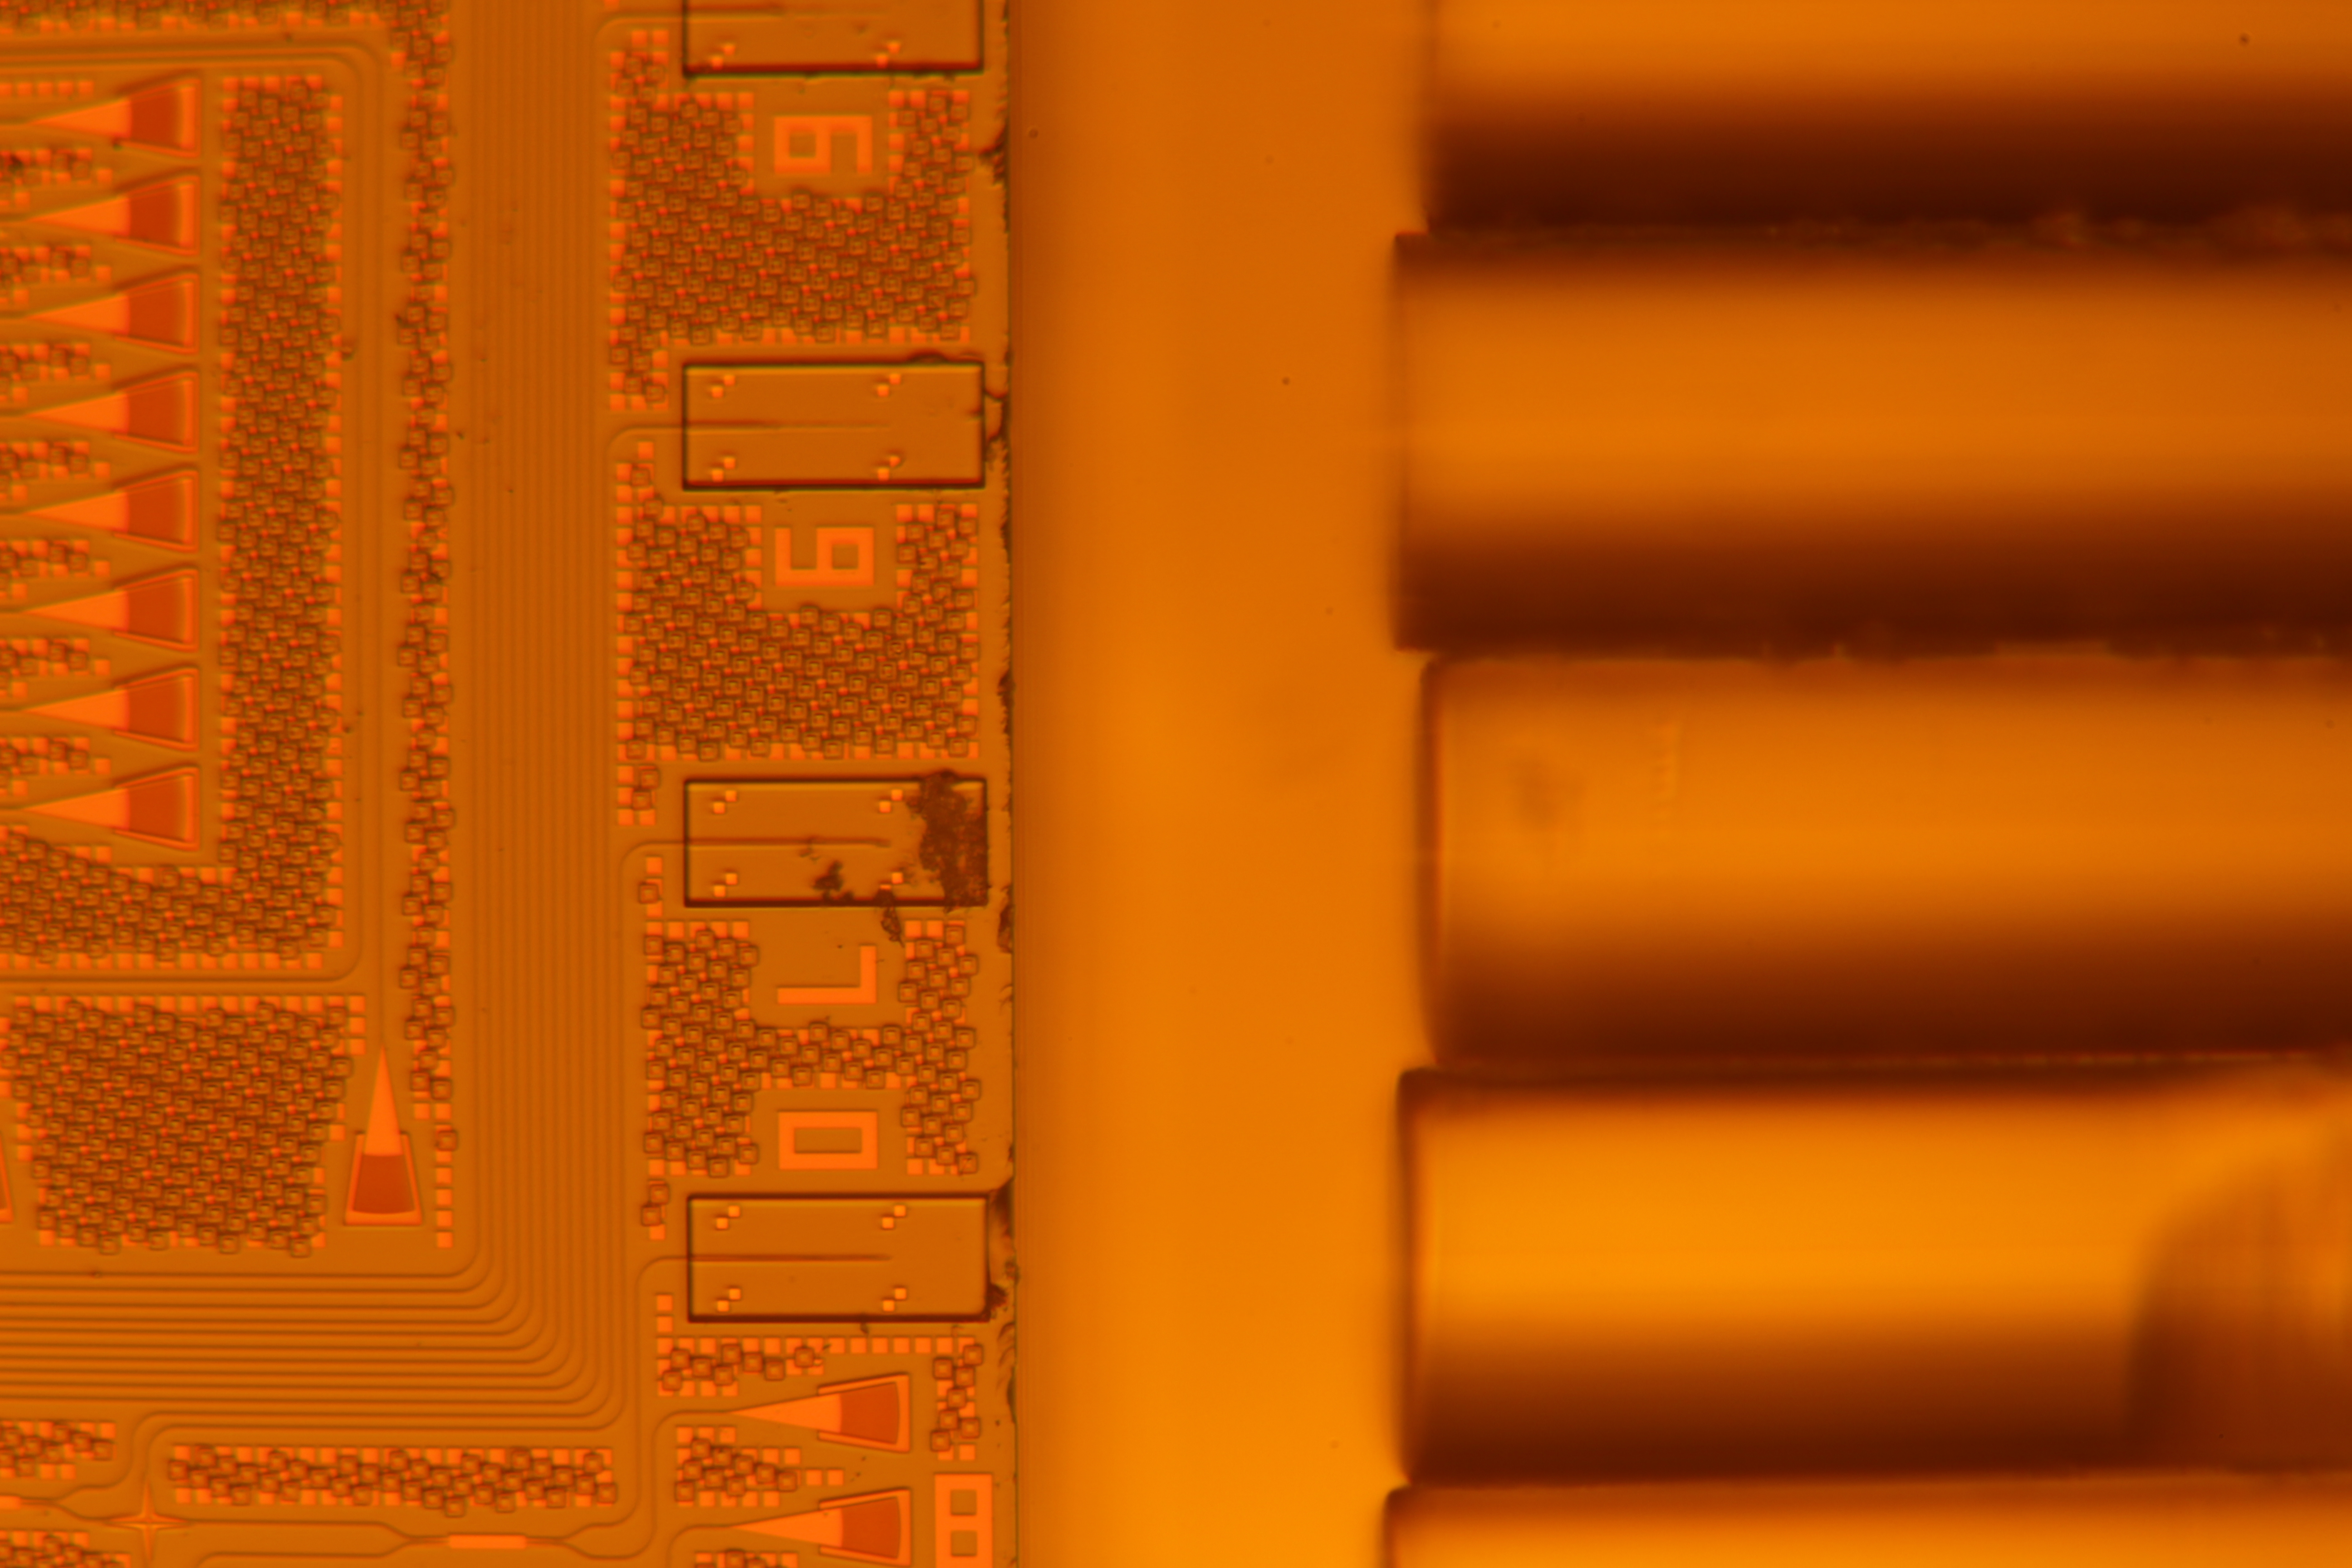
\includegraphics[width=0.42\textwidth]{lab/mcm01-01}} &
%\subfloat[Scratched pads]{{\label{fig:mcm1_AS2}}\includegraphics[width=0.42\textwidth]{lab/mcm01-02}} \\
%\subfloat[Large bend radius]{{\label{figmcm1_AS3}}\includegraphics[width=0.42\textwidth]{lab/mcm01-03}} &
%\subfloat[Misaligned PWB]{{\label{fig:mcm1_AS4}}\includegraphics[width=0.42\textwidth]{lab/mcm01-05}} 
%\end{tabular}
%\caption{MCM fabrication defects.}
%\label{fig:MCM1_AS}
%\end{figure}

%The first multi-chip module (MCM) was developed focusing on full optical paths, starting from the HCSEL and reaching the output single mode fiber, with small or undetectable (by immediate visual inspection) issues with the devices. The first issues found on the devices were broken tapers; dirt in the ports (figure \ref{fig:MCM1_AS1}); and scratches due to measurements or device handling (figure \ref{fig:MCM1_AS2}). During the PWB writing process, other unexpected errors occured, such as misalignments during the writing process and miscalculations of output port location (figure \ref{fig:MCM1_AS3} and \ref{fig:MCM1_AS4}). This was only found in the first MCM. Subsequent MCMs were visually inspected to avoid using SOH chips with noticeable damage in the tapers or close to the ports that could potentially hinder the writing of PWBs. 

%% ---------------------
%% | / Example content |
%% ---------------------

The main goal of the experimental section of this master thesis with respect to the multi-chip module is achieving homogeneous transmission across all the channels of a single device. This implies that the $V_\pi$ must also be consistent among all devices, and thus it can be considered that a single, optically-packaged transmitter is capable of transmitting data at the same rate in all its channels, and thus the aggregate data rate extrapolations is valid. The following modifications were considered in search for homogeneous transmission across all channels in a device.

\subsection{Integrated Gate-Voltage Chip Module}

Application of gate voltage was thoroughly analyzed by Alloatti in his thesis \cite{gateAlloatti12}, in order to enhance the electron and hole concentration at the semiconductor interface, and thus field enhancement inside the slot which produces a highly conductive electron accumulation layer to overcome the RC speed limitation of the slot. With the improvement of the performance by application of gate voltage of the multi-chip module, a second design featuring a layered submount as shown in figure \ref{fig:MCM2-SU}, in order to avoid electrical interference in the operation of the HCSEL, because the metallic substrate ties all the grounds of the chips to a common voltage level (i.e. ground). 

The submount differs from figure \ref{fig:MCM1-SUx} by the intermediate step of the submount between the HCSEL and the SOH chip. This provides an additional space of \SI{700}{\micro\meter} to place an intermediate dielectric layer between the HCSEL and the aluminum submount. This way, the gate voltage applied to the SOH will not interfere with the HCSEL operation, in the form of an electric field across the laser diode. The selected isolation layer is an alumina (\ce{Al2O3}) slab of \SI{633}{\micro\meter} with a \SI{3}{\micro\meter} layer of gold (\ce{Au}) on top. As noted by the work of Yoshimura \cite{AluminaYoshimura81}, the dielectric breakdown of alumina is well above the voltage levels utilized in this experiment and the dielectric constant $\epsilon_R=9.6$ is sufficient to avoid any electric field interacting with the laser chip. The rest of the setup was not modified.

\begin{figure}[!ht]
\centering
  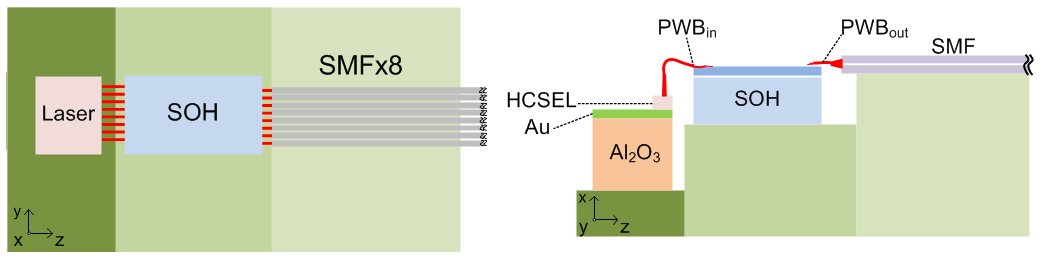
\includegraphics[width=0.9\textwidth]{visio/MCM2-SU}
  \caption{HCSEL isolation stack-up. A three-step aluminum mount is designed in-house to hold the three chips at different heights. An alumina submount with a thin gold layer is used as for the HCSEL submount. The SOH still lies on top of the aluminum mount, while the fibers are placed at the same location as previously.}
  \label{fig:MCM2-SU}
\end{figure}

\begin{table}[]
\centering
\begin{tabular}{@{}rrrrrrrrr@{}}
\toprule
Device                        & \multicolumn{1}{c}{1} & \multicolumn{1}{c}{2} & \multicolumn{1}{c}{3} & \multicolumn{1}{c}{4} & \multicolumn{1}{c}{5} & \multicolumn{1}{c}{6} & \multicolumn{1}{c}{7} & \multicolumn{1}{c}{8} \\ \midrule
Transmission {[}dBm{]}       & -22.8                  & -22.3                  & -23.0                  & -17.6                  & -44.8                  & -28.2                  & -32.9                  & -34.8                  \\
V$_\pi \cdot L$ {[}V$\cdot$mm{]} & 1.53                  & 1.64                  & 1.96                  & 1.47                  & 1.93                  & 1.40                  & 1.98                  & 1.46                  \\ \bottomrule
\end{tabular}
\caption{Transmission and $V_\pi \cdot L$ of MCM with HCSEL mounted on alumina submount summary.}
\label{tab:MCM2_sum}
\end{table}

Table \ref{tab:MCM2_sum} shows the most important figures obtained from the HCSEL isolation characterization. At first glance, there is an increase of V$_\pi$ and a very steep overall increase of the insertion loss, leading to suspicion of a process-related variations. Additionally, the HCSEL was observed to have worst parameters when in a non-metallic submount, effects which were briefly investigated in the form of the thermal roll-off observed in several HCSEL devices.
%The samples were analyzed and it was observed that there was a very visible contamination in the samples, depicted in figure \ref{fig:MCM2_contamination}. The particles were not suspected to be metallic since no electrical shorts were detected during the characterization, but the possible presence of sub-wavelength particles and air bubbles inside the slot were suspected as the main cause of the high insertion loss of the chips.

%\begin{figure}[!ht]
%\centering
%  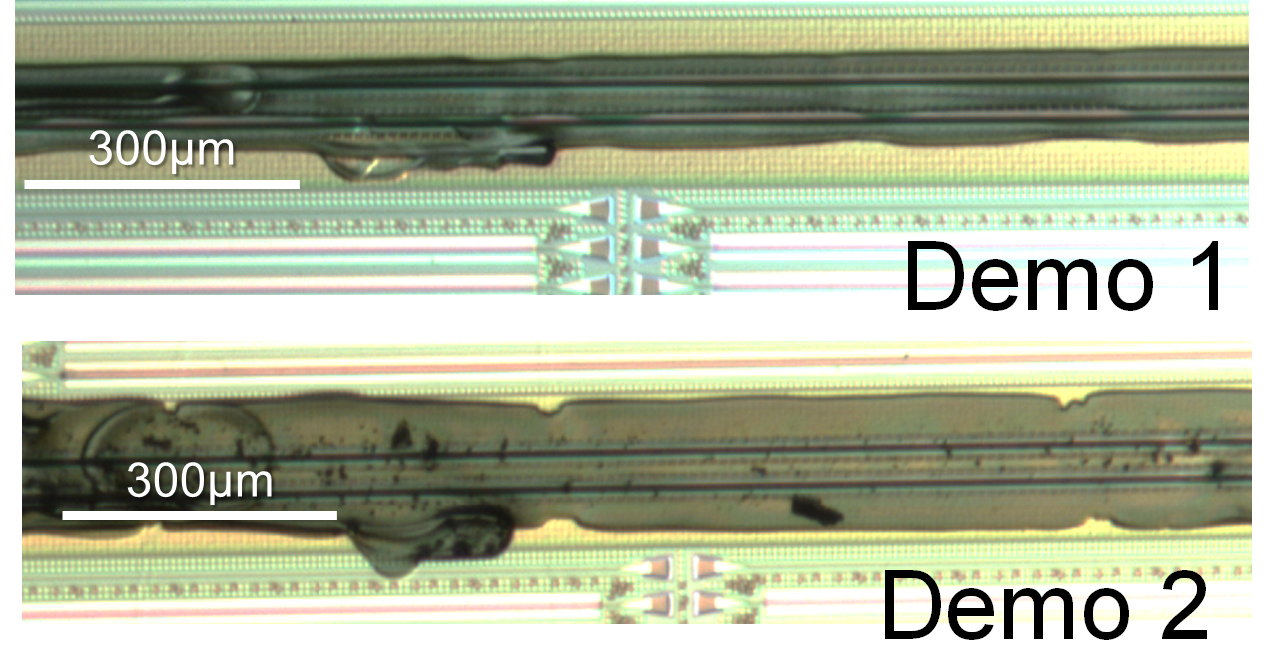
\includegraphics[width=0.9\textwidth]{lab/mcm2_contamination_2}
%  \caption{EO polymer contamination. Demo 1 shows the initial microscope images taken in the lab, with a visibly homogeneous polymer on top of the slots. Demo 2 shows a device where there are black spots in the polymer, suspected to also contain sub-wavelength particles that deposit inside the slot and cause higher losses in the slot.}
%  \label{fig:MCM2_contamination}
%\end{figure}

%\subsubsection{Laser Threshold Current-Temperature Dependence}
%\label{sec:Evaluation:lasertemp}

%For one demonstrator, the spacer substrate submount used for the laser chip was substituted from a \SI{500}{\micro\meter} copper (\ce{Cu}) slab to a \SI{600}{\micro\meter} alumina (aluminum oxide, \ce{Al2O3}) substrate. 

The thermal conductivity of \ce{Al2O3} is 18,25 and \SI{35}{\watt/\meter\kelvin}, depending on its composition (94\%,96\% and 99.5\%, respectively). The thermal conductivity of \ce{Cu} is \SI{385}{\watt/\meter\kelvin}, according to \cite{TempYoung92}. The common carrier substrate is made of aluminum (\ce{Al}) with a thermal conductivity of \SI{205}{\watt/\meter\kelvin}. The thermal conductivity difference between alumina and copper is almost tenfold. Three very important changes to the operation conditions of the laser under a change of the submount substrate: %When analyzed as a heat sink, the heat flow can be modeled with static thermal conduction equation (why?!?!?!?!?!?!?!?!?):
%Figure \ref{fig:MCM12_LI} shows the LI curves of the operational laser chips plotted with MATLAB. The graph shows t

%\begin{align}
%k \nabla^2 T + Q = 0
%\end{align}

%Where $k$ is thermal conductivity  and $Q$ is the power density of heat. The heat sink is assumed to be a thermal reservoir at the %surface and heat extraction by air negligible, $\nabla T=0$. With thermal power density $q$ defined as:

%\begin{align}
%q = -k \nabla T
%\end{align}

%And the power density of heat can be considered constant due to the size difference of the laser chip and the heat sink. This can be easily solved by FEM. (Do the FEM) The analysis shows that higher thermal conductivity reduces temperature, but it would be expected to have an increased temperature in the laser surface, and thus a change of the operating current. 


\begin{itemize}
\item Increase of the mean threshold current of each chip of \SI{2}{\milli\ampere}
\item Decrease of the mean slope efficiency of \SI{0.18}{\milli\watt/\milli\ampere}
\item Decrease of the mean light output power of \SI{1.48}{\milli\watt} or \SI{1.7}{\decibel} attenuation
\end{itemize}

The performance decrease was due to the increase of temperature of the laser diode chip (and thus increased junction heating) due to reduced thermal conductivity of the heat sink\footnote{Thermal rollover is due to the positive feedback loop between increasing laser core temperature and threshold current density due to thermal back-filling; and Stark shift in the conduction band structure decreasing the optical dipole matrix element leading to reduced internal quantum efficiency \cite{HowardLDTher08}.}. %The thermal rollover is only observed in two lasers of MCM1 and a more consistent overall behavior in the HCSELs of MCM2. This results must be taken, nonetheless, as a naive intuition, since there was no specific thermal control implemented in the experiment, although the testing conditions and setup was relatively unchanged (i.e. no external factors were abruptly changed such as setup location and configuration, room temperature, testing time, etc.) between experiments.


%\begin{figure}[!ht]
%\centering
% \includegraphics[width=0.8\textwidth]{figs/PI_laserA4144_ith_iop_demo001-2}
%  \caption{MCM demo laser chip LI curves.}
%  \label{fig:MCM12_LI}
%\end{figure}


In the literature, the threshold current of \ce{InP} laser diodes have been analyzed for temperature dependence by Ishikawa \cite{IshikawaTempLD91}, more rigorously for \ce{GaAs} quantum well laser diodes by Menzel \cite{MenzelTempLD95} and in a simplified approximation from Nakwaski \cite{NakwaskiTempLD83}, there is no specific research that directly compares the thermal resistance of alumina and copper. %Nonetheless, a model proposed by Zhao \cite{ZhaoTempLD06} can be used for solving a simple 2D model that would provide a good approximation of the best structure for improving the thermal performance. s 

%The thermal resistance relates the dimensions of a heatsink with its thermal conductivity. For alumina:

%\begin{align}
%R_{th} = \frac{L}{k} = \frac{\SI{18.25}{\watt/\meter\kelvin}}{}
%\end{align}


%http://ieeexplore.ieee.org/stamp/stamp.jsp?arnumber=4098422

%To do:
%\begin{itemize} 
%\item Discussion of electrically-isolated current source*
%\item Discussion of HF Dip
%\item Discussion of air exposure and improvement of successful device transmission yield
%\end{itemize}
%\subsection{Process modification}

\begin{figure}[!ht]
\centering
  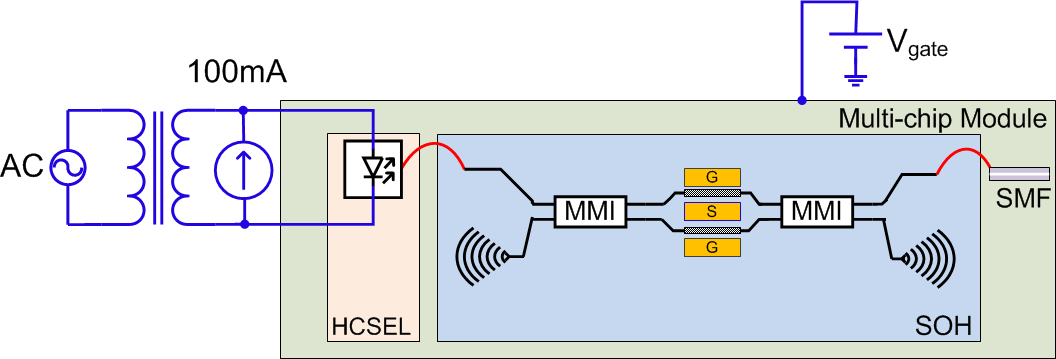
\includegraphics[width=0.9\textwidth]{visio/MCM3-SU}
  \caption{Gate voltage investigation setup for HCSEL changes in-operation effects. An electrically isolated current source is used to power the HCSEL and a high voltage source is used to apply gate voltage to the ground plane of the MCM.}
  \label{fig:mcm3-su}
\end{figure}

Further experimental setups were used in order to find if the electrical isolation of the HCSEL is necessary. The setup is shown in figure \ref{fig:mcm3-su}, where the current source LDX-3207 with an isolated output is used to inject current to the HCSEL chip, while a high voltage source applies voltage to the reference plane (i.e. the aluminum mount) of the MCM. No significant threshold current, operation power or spectral shift is observed in the HCSEL after application of gate voltage for 1, 3 and 5 minutes. Thus, the application of gate voltage was deemed safe for operating HCSELs for the following experiments, and electrical isolation of the HCSEL is no longer required.

%\subsection{Transmission Homogenization}
%A new module was developed in order to correct the bad transmission found earlier.
%The full process is repeated with successful writing on all devices, from pre-characterization to poling. The devices are tested in the transmission setup, using a simple GC-MZM-GC setup. The results are summarized in table \ref{tab:MCM3_sum}. %Device 7 had a transmission below detection threshold ($P_\text{launch}<\SI{-90}{\decibel}$) so no figure was obtained. Devices 6 and 8, as pointed out already, are combined ports so a free spectral range behavior can be observed. 

% Please add the following required packages to your document preamble:
% \usepackage{booktabs}
%\begin{table}[]
%\centering
%\caption{My caption}
%\label{my-label}
%\begin{tabular}{@{}rcccccccc@{}}
%\toprule
%Device                  & 1                        & 2                        & 3                        & 4                        & 5                        & 6                        & 7                        & 8                        \\ \midrule
%Insertion Loss {[}dB{]} & \multicolumn{1}{r}{29.2} & \multicolumn{1}{r}{73.4} & \multicolumn{1}{r}{41.2} & \multicolumn{1}{r}{10.7} & \multicolumn{1}{r}{20.2} & \multicolumn{1}{r}{51.7} & \multicolumn{1}{r}{$>90$} & \multicolumn{1}{r}{10.26}
%\end{tabular}
%\caption{MCM3 Summary}
%\label{tab:MCM3_sum}
%\end{table}

%\begin{figure}[!ht]
%\centering
%  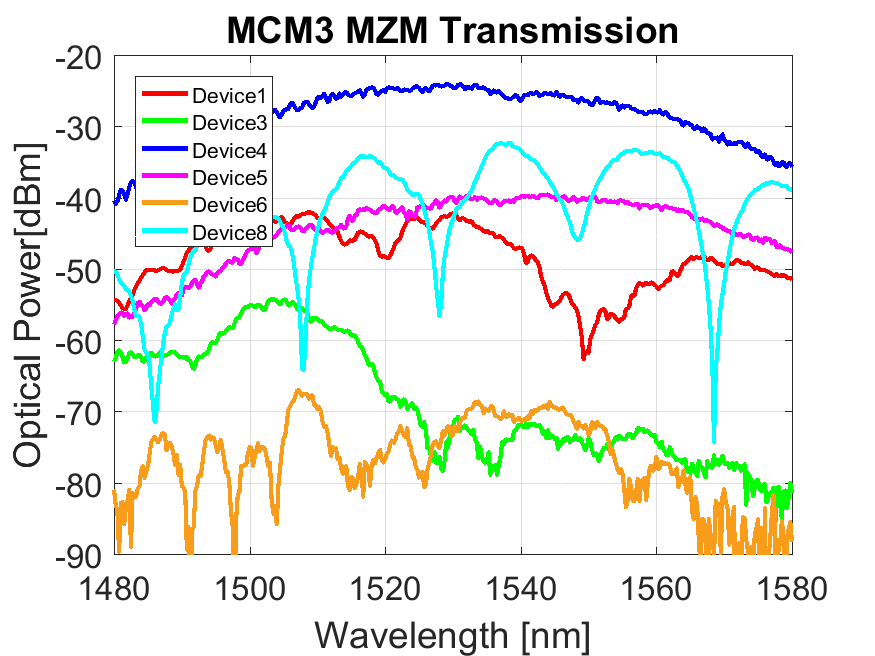
\includegraphics[width=0.9\textwidth]{figs/MCM3/MZM_Transmission_demo003}
%  \caption{MCM3 Transmission.}
%  \label{fig:MCM3_TX}
%\end{figure}

%One possible explanation for the poor performance is having the devices unproperly poled: As mentioned in the theoretical framework section \ref{{sec:thbkgd:poltechs}}, if the electro-optic material is not poled, the instrinsic anisotropy of the polymer reduces charge mobility in the polymer, and thus the interaction of the RF and the optical field is severly reduced, or in the worst case scenario, neglible. A re-poling of the EO polymer was made to corroborate the effect of bad poling. Devices 2 and 3 showed transmission below threshold so no curve was recorded, while devices 1 and 4 showed no specific improvement, with the appearance of new transmission dips but improvement in other wavelengths. The process   %This lead to the assumpion that there is a  in the devices, such as sub-wavelength particles that lead to scattering, and thus requiring a change in the processing scheme.


%\begin{figure}[!ht]
%\centering
%  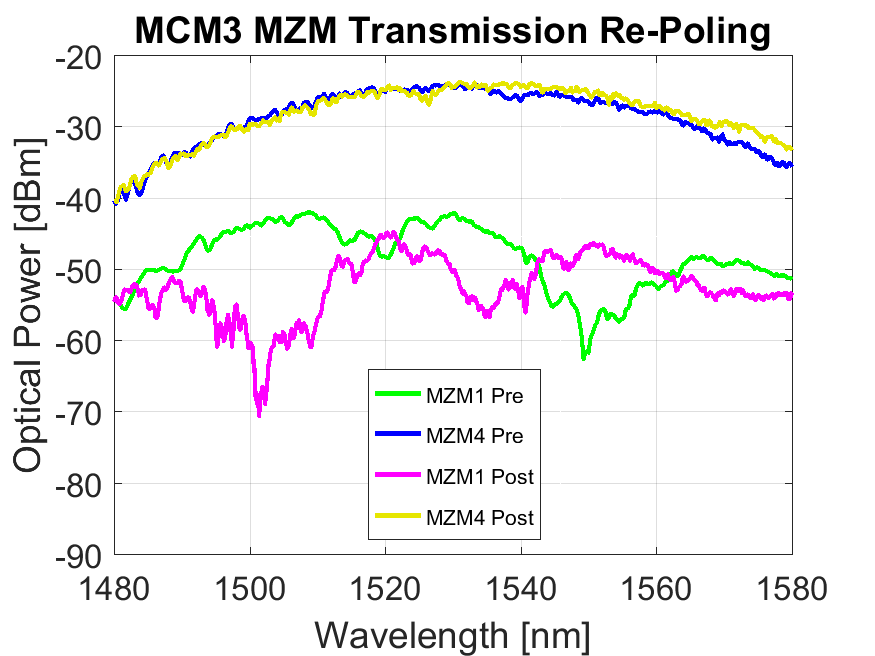
\includegraphics[width=0.9\textwidth]{figs/MCM3/MZM_Transmission_PrePostPoling_demo003}
%  \caption{MCM3 Re-poling (pre-poling and post-poling shown above).}
%  \label{fig:MCM3_TX_repol}
%\end{figure}

In order to modify the processing scheme, additional investigation was done on the HCSEL portion, since avoiding air exposure after HF dip is of vital importance, when the SOH chip has its PMMA overcoating and thin \ce{SiO2} removed, and thus possibly exposing the slot to external contamination. A HCSEL sample chip was then fully processed as if mounted for a multi-chip module (i.e. pre-characterization, IP dip exposition, PGMEA/isopropanol solvent bath and critical point drying), and then dipped in HF, to detect any possible changes in the electrical or optical behavior of the chip. The HCSEL was characterized in light power output and spectrum, and no significant changes were observed in its wavelength peaks or operation power ($\Delta\bar{f}=\SI{0.1}{\nano\meter}$ and $\bar{\Delta P_{op}}=\SI{0.45}{\milli\watt}$, respectively). The measurements were not done with thermal stabilization. Only minor aesthetic changes were observed in the HCSEL chip, such as the faded color coating and removal of small particles on the chip surface.

% \begin{figure}[!ht]
%\centering
%\begin{tabular}{cc}
%\subfloat[Microscope Image]{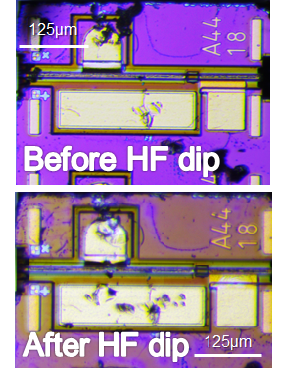
\includegraphics[width=0.40\textwidth,valign=m]{lab/HF_dip2}\label{fig:HF1}} %&
%\subfloat[Spectral Shift]{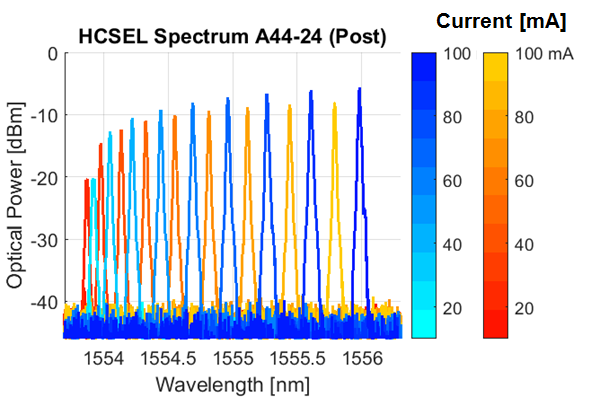
\includegraphics[width=0.5\textwidth,valign=m]{figs/HF_dip_spectralshift}\label{fig:HF2}} \\
%\end{tabular}
%\caption{HF dip effects on HCSEL. Color fading of the HCSEL coating can be observed after dipping. %Figure \ref{fig:HF2} shows the spectral shift before (red-yellow) and after (blue) dipping.
%}
%\label{fig:HFdips}
%\end{figure}

\begin{figure}[!ht]
\centering
  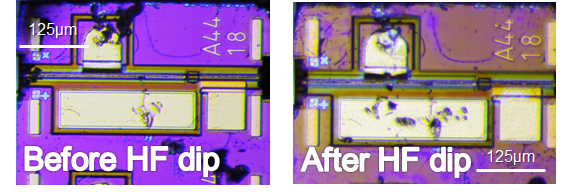
\includegraphics[width=0.8\textwidth]{lab/HF_dip}
  \caption{HF dip effects on HCSEL. Color fading of the HCSEL coating can be observed after dipping.}
  \label{fig:HFdips}
\end{figure}

%\begin{figure}[!ht]
%\centering
%  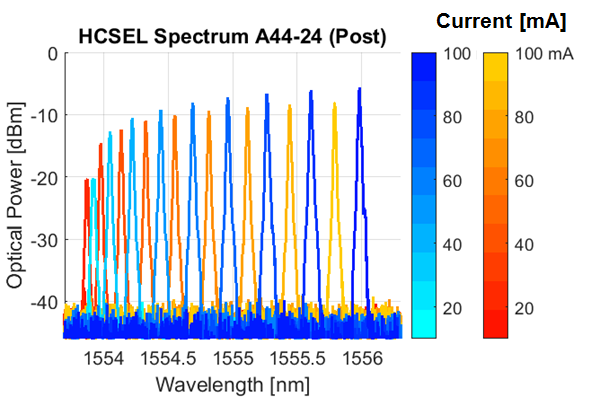
\includegraphics[width=0.8\textwidth]{figs/HF_dip_spectralshift}
%  \caption{HCSEL microscope view before and after HF dip.}
%  \label{fig:HF_Dip_specshift}
%\end{figure}



%\begin{itemize}
%\item Results from Demo2 (bad transmission)
%\item Results from Demo3 (HF dip, repoling, )
%\item Results from Demo4 (Characterization, results obtained)
%\item Results from Demo5 (Characterization, working still on 02.05.2017)
%\end{itemize}

%Refractive index InP 
%@1.55µm n = 3.1649 dn/dλ = -0.11135 µm-1 ng = 3.3375 GVD = 1739.6 fs2/mm D = -1363.9 ps/(nm km)
%Pettit and Turner 1965 


% Please add the following required packages to your document preamble:
% \usepackage{booktabs}
%\begin{table}[]
%\centering
%\begin{tabular}{@{}lllllllllll@{}}
%\toprule
%$\Delta \lambda$ {[}nm{]} & \multicolumn{10}{c}{Current {[}mA{]}}                                         \\ \midrule
%Device                    & 10    & 20    & 30    & 40    & 50    & 60    & 70    & 80    & 90    & 100   \\
%1                         & 0,563 & 0,155 & 0,091 & 0,012 & 0,137 & 0,293 & 0,46  & 0,71  & 0,986 & 1,293 \\
%2                         & 0,014 & 0,044 & 0,038 & 0,046 & 0,039 & 0,053 & 0,062 & 0,079 & 0,13  & 0,121 \\
%3                         & 0,042 & 0,037 & 0,031 & 0,01  & 0,022 & 0,018 & 0,052 & 0,074 & 0,119 & 0,106 \\
%4                         & 0,007 & 0,032 & 0,021 & 0,011 & 0,003 & 0,034 & 0,081 & 0,102 & 0,109 & 0,144 \\
%5                         & 0,008 & 0,008 & 0,019 & 0,028 & 0,031 & 0,012 & 0,02  & 0,013 & 0,042 & 0,075 \\
%6                         & 0,001 & 0,001 & 0,003 & 0,01  & 0,013 & 0,029 & 0,085 & 0,111 & 0,136 & 0,171 \\
%7                         & 0,028 & 0,028 & 0,035 & 0,04  & 0,037 & 0,04  & 0,031 & 0,028 & 0,016 & 0,006 \\
%8                         & 0,039 & 0,048 & 0,072 & 0,085 & 0,118 & 0,138 & 0,146 & 0,15  & 0,165 & 0,191 \\ \bottomrule
%\end{tabular}
%\caption{Wavelength shift before and after HF dip per current step in HCSEL.}
%\label{tab:lambdashift_HFdip}
%\end{table}

\subsection{Modified Process Flow and Results}

\begin{figure}[!ht]
\centering
  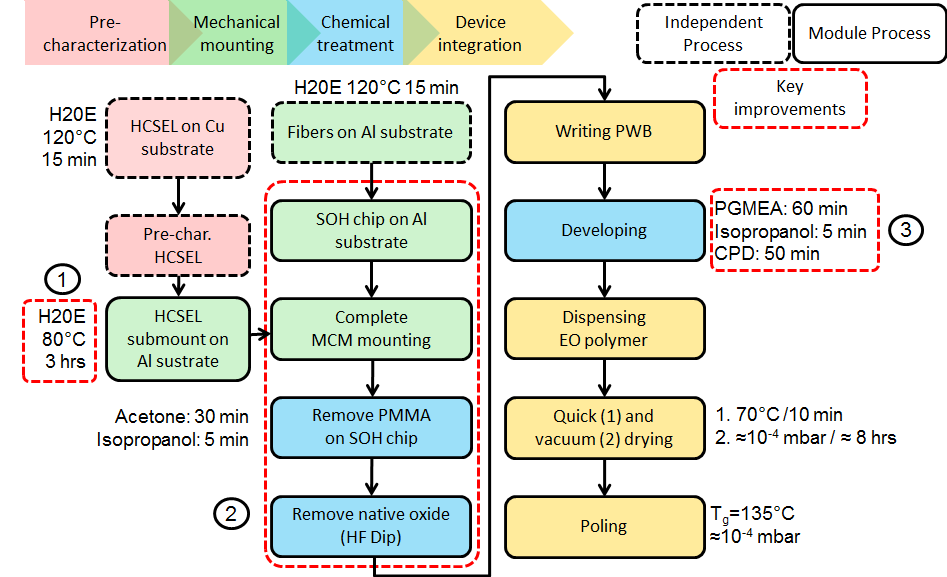
\includegraphics[width=0.9\textwidth]{visio/final_process}
  \caption{Final process flow for multi-chip module (MCM) production. The key changes rely on complete MCM mounting and further process the whole device by dipping in acetone and HF for PMMA \ce{SiO2} dissolution, respectively, and thus avoiding slot exposure to the environment.}
  \label{fig:fproc}
\end{figure}

The final process flow developed in this master thesis featuring consistent $V_\pi$ and transmission is shown in figure \ref{fig:fproc}. The key improvements done to the process are the following:

\begin{enumerate}
\item \textbf{HCSEL process modification:} With the knowledge that there is no effect in the HCSEL in the HF dip chemical treatment, the possibility to process the whole module through the removal of PMMA and native silicon oxide was deemed reliable. 
\item \textbf{SOH mounting process modification:} This meant that the SOH device would also have to be reliable during the mechanical mounting of the HCSEL. The thermal curing of the epoxy used can be reduced in temperature at the cost of increasing the exposure time. This is critical to avoid the glass transition temperature of PMMA, sitting between \SI{85}{\celsius} and \SI{165}{\celsius}, so the temperature is chosen below the lowest limit to avoid hardening of PMMA which can change the dissolving dynamics during the following processes.
\item \textbf{PWB development modification:} The time in which the module sits in PGMEA and isopropanol is increased to ensure there are no traces of IP-dip inside the slot after the PWB writing. This was taken as a cautionary measure, considering the previously observed correlation between the exposure of the slot and the final EO polymer deposition.
\end{enumerate}

\begin{figure}[!ht]
\centering
  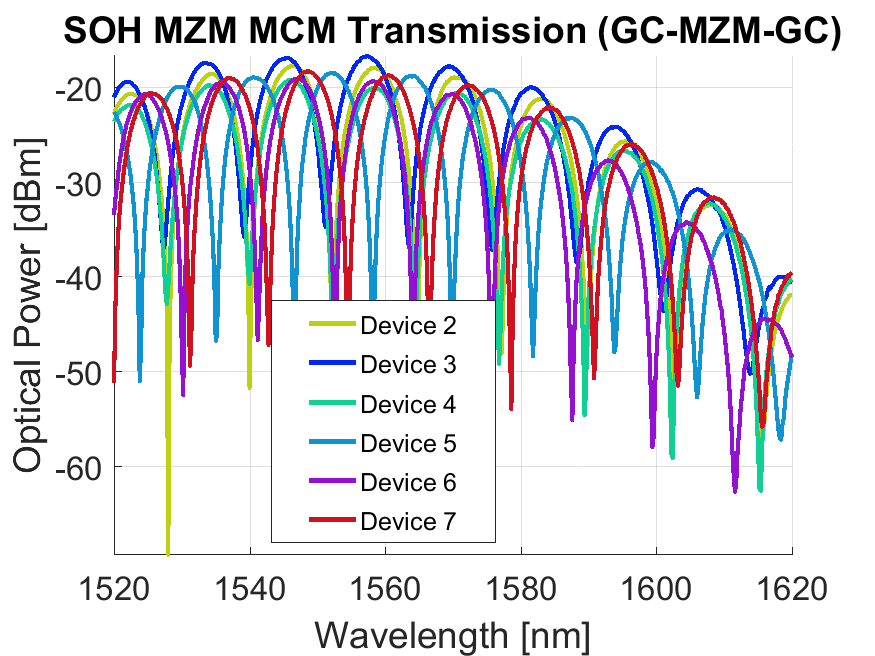
\includegraphics[width=0.85\textwidth]{figs/MCM4/MCM4_IL_measured_demo004}
  \caption{Improved process flow MCM transmission function. Devices 1 and 8 are not accesible in IQ configuration. The grating coupler transmission function is still visible.}
  \label{fig:MCM4_TX}
\end{figure}

\begin{table}[]
\centering
\begin{tabular}{@{}rrrrrrrrr@{}}
\toprule
Device                        & \multicolumn{1}{c}{1} & \multicolumn{1}{c}{2} & \multicolumn{1}{c}{3} & \multicolumn{1}{c}{4} & \multicolumn{1}{c}{5} & \multicolumn{1}{c}{6} & \multicolumn{1}{c}{7} & \multicolumn{1}{c}{8} \\ \midrule
V$_\pi \cdot L$ {[}V$\cdot$mm{]} & N/A                  & 1.36                  & 1.37                 & 1.3                  & 1.36                  & 1.36                  & 1.32                  & N/A                  \\ \bottomrule
\end{tabular}
\caption{$V_\pi \cdot L$ measurement of improved process flow MCM. Devices 1 and 8 are not accessible in the IQ configuration.}
\label{tab:MCM2_sum}
\end{table}

The above changes were implemented in the final demonstrator, a \SI{1}{\milli\meter} IQ modulator. The module was processed in a way that avoided air exposure of the slots until the EO polymer deposition, meaning that between the HF dip and the PWB writing, the chip was sealed and transported between clean rooms without exposition to light or air. The transmission of 6 MZM is plotted in figure \ref{fig:MCM4_TX}, and it shows a very consistent transfer function across all modulators. The transmission of the grating coupler can still be observed, which was not recorded at the moment of initial characterization due to time constraints. The former results  that avoiding air exposure of the slots gives a homogeneous transmission across the device due to minimal external agents introduced to the slot.



\subsection{Thermal Roll-off Analysis}
Thermal roll-off was observed in few HCSEL units with no specific correlation to external damage due to handling, such as scratching of the anode or cathode pads; damage of the ridge waveguide due to scratching; or general external structural characteristics of the HCSEL. Buried heterostructure laser diodes (such as the HCSEL used here), exhibit gradual performance degradation due to possible defects created during the mesa etch and regrowth of the sidewall of the active and cladding layer \cite{SwinglerThermal14}. Thus, the  morphology of the HCSEL layers is of vital importance to understand the roll-off phenomenon.

\begin{figure}[!ht]
\centering
\begin{tabular}{cc}
\subfloat[LI Curve]{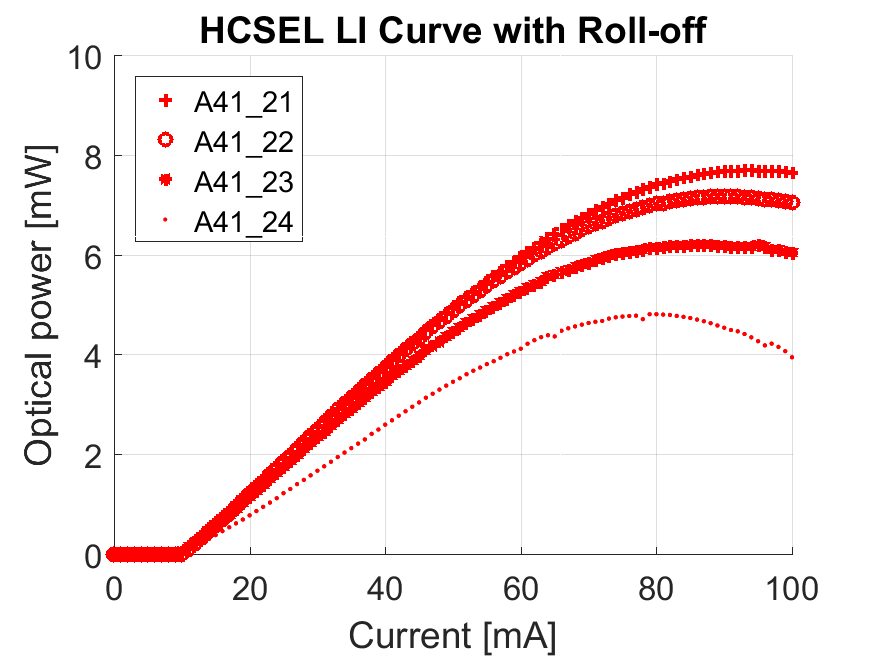
\includegraphics[width=0.5\textwidth,valign=m]{figs/MCM4/LI_laserA41_ith_iop_demo004}\label{fig:LI_TR_2}} &
\subfloat[Spectrum]{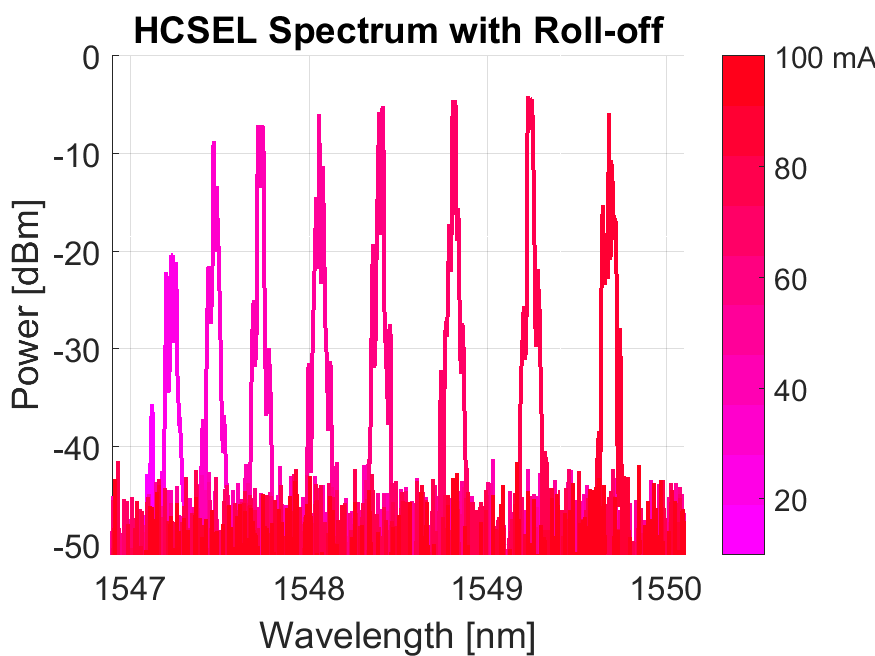
\includegraphics[width=0.5\textwidth,valign=m]{figs/MCM4/SPK/HCSEL1_Spectrum_demo004_PRE}\label{fig:Df_SPK_2}}  \\
\end{tabular}
\caption{HCSEL Roll-off behavior. A HCSEL with increasingly prominent thermal roll-off is pre-characterized in light-current and spectral configurations.}
\label{fig:HCSELTR_rolloff}
\end{figure}

A quantitative but indirect approach to observe such behavior is depicted in the following. The spectrum of HCSEL arrays were recorded during the pre-characterization of the devices, paying special attention to those chips which show thermal roll-off. 

\begin{figure}[!ht]
\centering
\begin{tabular}{cc}

\subfloat[Wavelength shift]{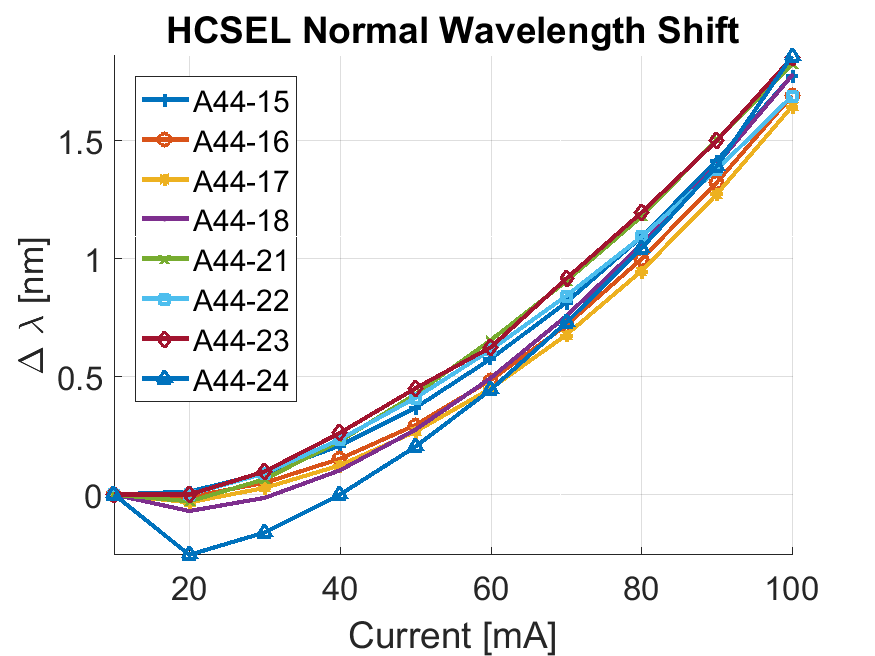
\includegraphics[width=0.5\textwidth,valign=m]{figs/MCM3/HF_Dip/SPK/HCSEL8_Spectrum_demo003_wlshiftPREPROC}\label{fig:Df_SPK}} &
\subfloat[Wavelength peaks]{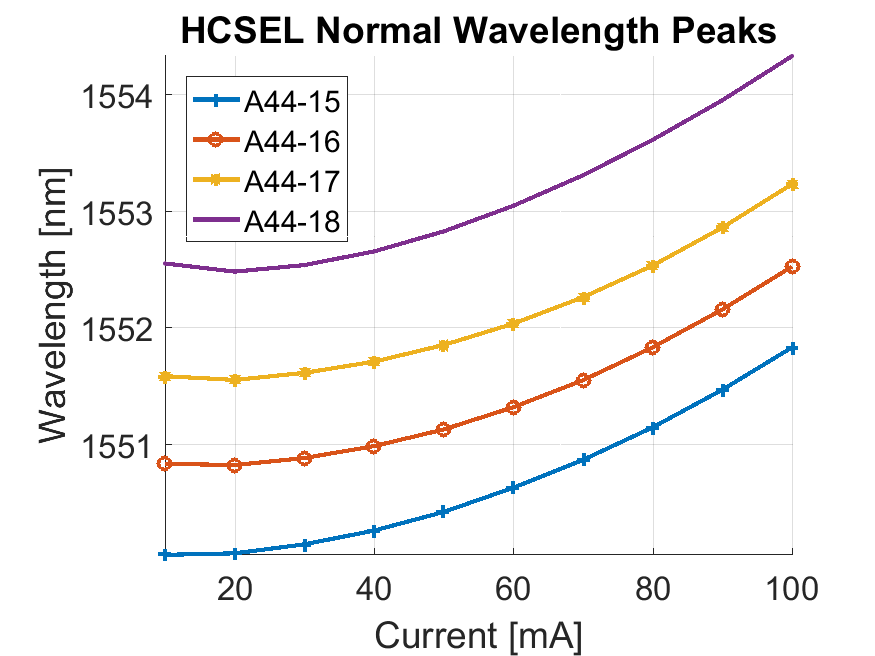
\includegraphics[width=0.5\textwidth,valign=m]{figs/MCM3/HF_Dip/SPK/HCSEL8_Spectrum_demo003_wlshiftPREPROC_peaks1}\label{fig:LI_TR}}  \\
\end{tabular}
\caption{HCSEL normal condition behavior.}
\label{fig:HCSELTR_normal}
\end{figure}

In figure \ref{fig:HCSELTR_normal}, The behavior of a normally-operating HCSEL is shown. Figure \ref{fig:Df_SPK} shows the wavelength shift that occurs during a current change of $\Delta i = \SI{10}{\milli\ampere}$. In figure \ref{fig:LI_TR}, the wavelength peaks can be observed for each HCSEL array and it is also notable that the wavelength peak spacing is consistent across the devices, and thus, there is no wavelength overlap .

\begin{figure}[!ht]
\centering
\begin{tabular}{cc}
\subfloat[Wavelength shift]{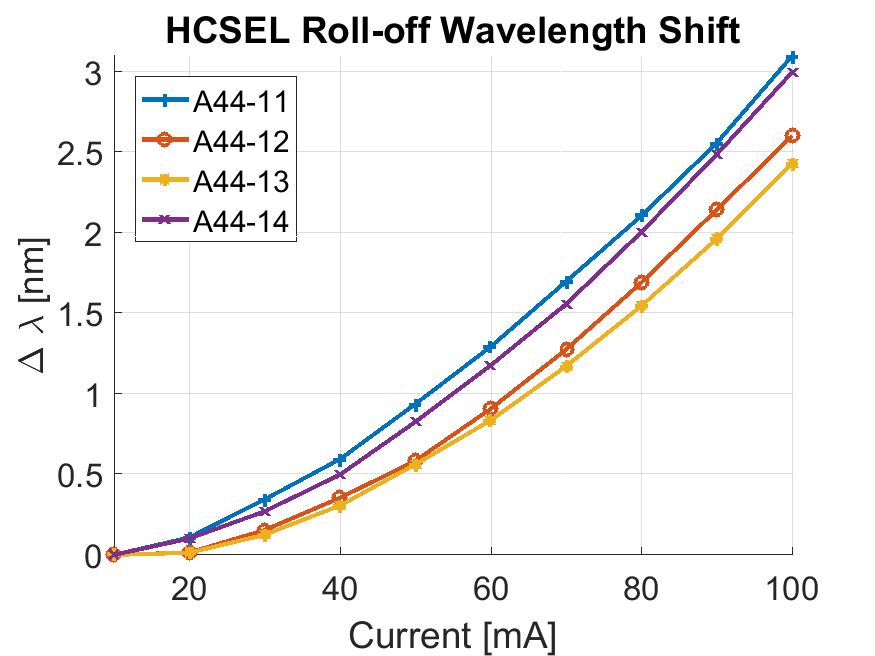
\includegraphics[width=0.5\textwidth,valign=m]{figs/MCM4/SPK/HCSEL4_Spectrum_demo001_wlshiftHCSEL4_Spectrum_demo00}\label{fig:Df_SPK4}}  &
\subfloat[Wavelength peaks]{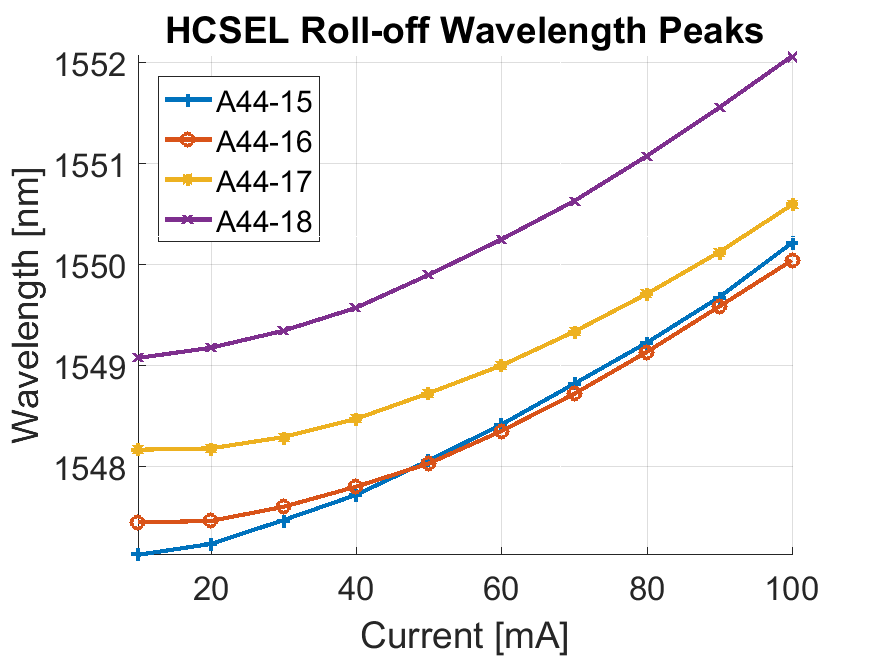
\includegraphics[width=0.5\textwidth,valign=m]{figs/MCM4/SPK/HCSEL4_Spectrum_demo001_wlshiftPREPROC_peaks1HCSEL4_Spectrum_demo00}\label{fig:Df_SPK5}}  \\
\end{tabular}
\caption{HCSEL Roll-off relative shift and peaks.}
\label{fig:HCSELTR_rolloff_peaks}
\end{figure}

In the case where a HCSEL features heavy roll-off, such as that in \ref{fig:HCSELTR_rolloff}, the LI curve shows increasingly high thermal roll-off, and the spectrum of the HCSEL that has the worst case roll-off. As expected, spectral hole burning is observed. It is however more interesting to see the relative shift and peaks in the case of heavy roll-off, as observed in figure \ref{fig:HCSELTR_rolloff_peaks}, with an increase of the slope in the relative wavelength between current steps, and a heavier red shift of the wavelength of the laser as current is increased. There is also a very noticeable overlap of the wavelength peaks, which makes the HCSEL array no longer reliable for applications such as WDM, because of the very likely overlap of wavelengths in a combined channel.

The spectral shifting of a HCSEL due to increased temperature can be correlated to the refractive index change in the buried heterostructure, through the relation \cite{BainTemp10}:

\begin{align}
 \frac{d \lambda}{d T} \propto \frac{d \tilde n}{dT}
\end{align}

And thus, as postulated previously, a slight structural change in the manufacturing of the HCSELs can thus show that a change of the thermal operation of the HCSEL, indicates a change of the refractive index inside the buried heterostructure, and thus, defects in the layer stack-up of the HCSEL. Specific structural analysis can be done with SEM pictures of the internal structure of the HCSEL, but such studies are outside of the scope of the work in the present master thesis. This provides some insights on the thermal roll-off phenomenon in HCSEL chips, which is not related to external structural issues but from the fabrication process of the device itself.